
%|  Name  | TODO | ONGOING | DONE |
%|--------|------|---------|------|
%| Dana   | x    |         |      |
%| Gerd   | x    |         |      |
%| Glenn  | x    |         |      |
%| Jordan | x    |         |      |
%| Luke   | x    |         |      |
%| Matt   |      |   x     |      |
%| Neil   | x    |         |      |
%| Scot   | x    |         |      |

An overview of HDF5 library modules' locations is shown in Figure~\ref{fig:module-location}.

\begin{landscape}
\begin{sidewaysfigure}[h!]
\centering
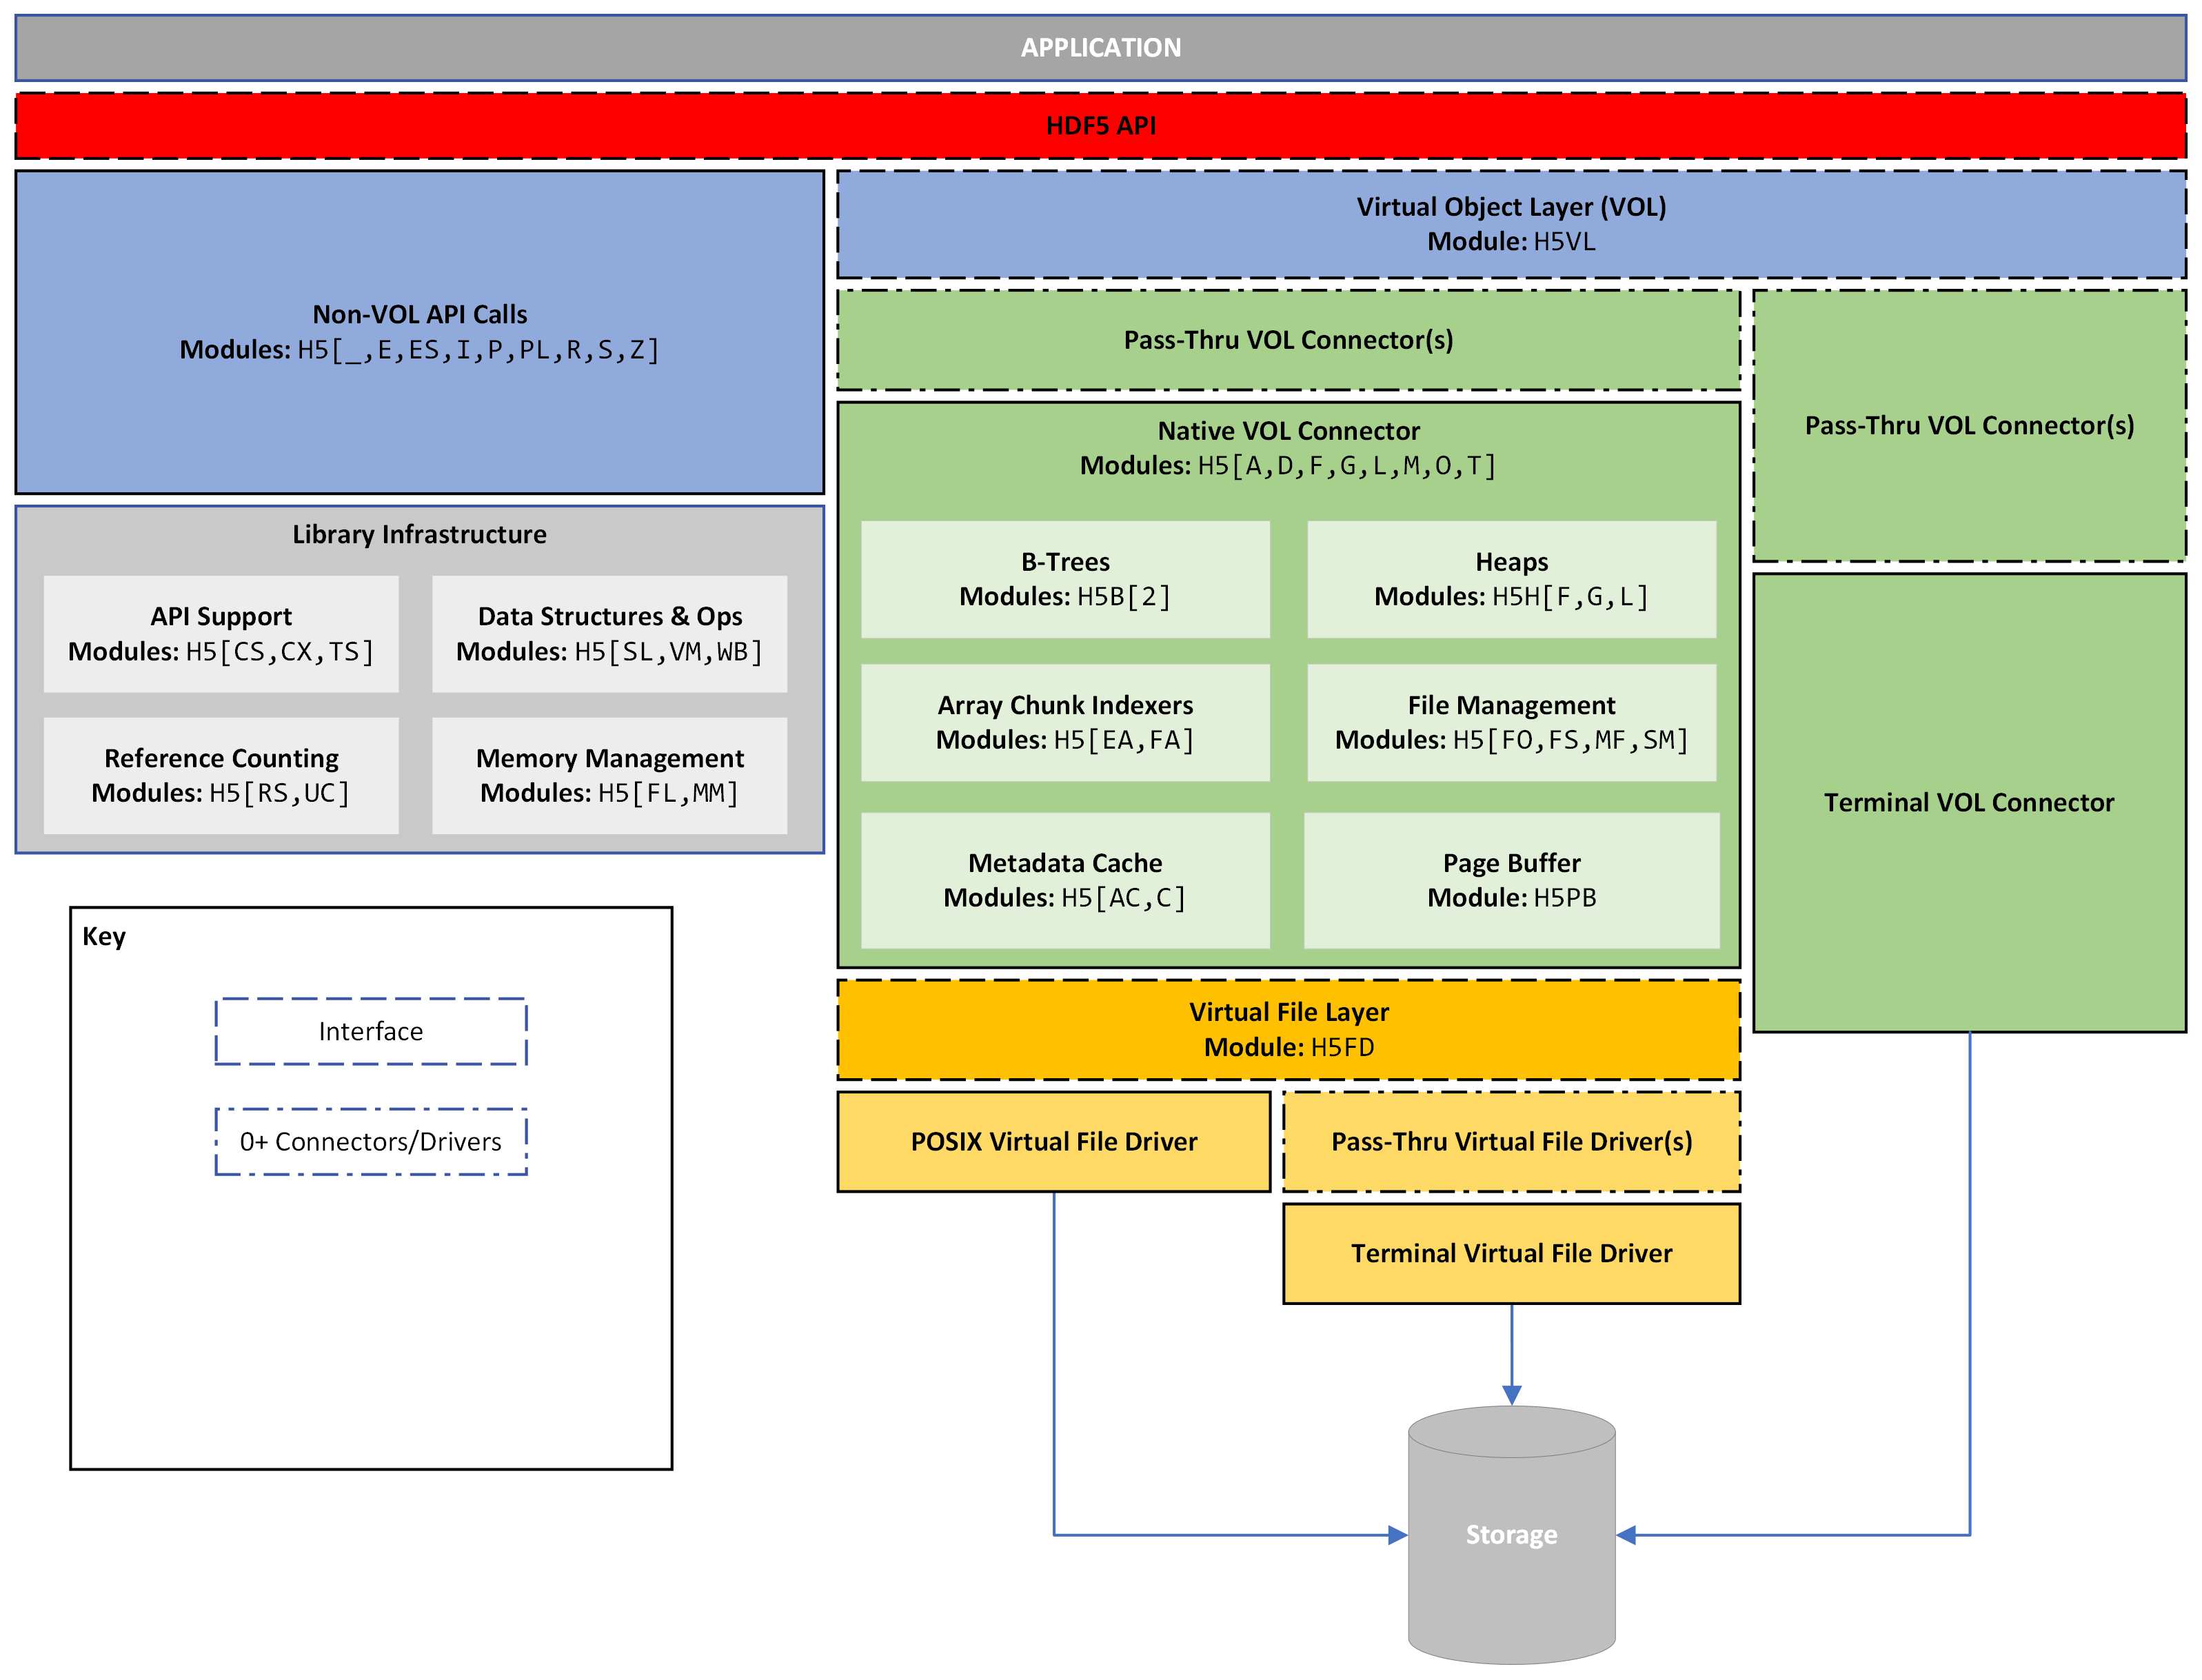
\includegraphics[scale=0.74,angle=90]{images/HDF5 library canvas.png}
\caption{The "location" of HDF5 library modules.\label{fig:module-location}}
\end{sidewaysfigure}
\end{landscape}

%\subsection{General Library Infrastructure (\texttt{H5})}
%\todo[inline]{Owner: ??? -- Priority: Low -- Effort: S}

\subsection{File Memory Allocation (\texttt{H5MF})}

%|  Name  | TODO | ONGOING | DONE |
%|--------|------|---------|------|
%| Dana   | x    |         |      |
%| Gerd   | x    |         |      |
%| Glenn  | x    |         |      |
%| Jordan | x    |         |      |
%| Luke   | x    |         |      |
%| Matt   |      |         |  x   |
%| Neil   | x    |         |      |
%| Scot   | x    |         |      |

%\todo[inline]{Owner: Matt -- Priority: Medium -- Effort: S -- Completion: 100\%}


The file memory management module \texttt{H5MF} is one of the major clients of the \Gls{fsm} module \texttt{H5FS}. Many file memory management routines act as wrappers around corresponding \Gls{fsm} operations. \texttt{H5MF} also manages some higher-level memory processes, such as paged aggregation (if enabled) and free space aggregators (if paged aggregation is disabled).

\begin{itemize}

    \item Allocation Types

\texttt{H5MF} uses the type of allocation requested to determine which type of \Gls{fsm} to create, open, or use for each file memory request. Allocation type indicates what type of low-level file element the allocated memory block is for. The allocation types are superblock, B-tree, raw data (\texttt{DRAW}), global heap, local heap, and object header. All of these allocation types besides 'raw data' are metadata.

    \item Free Space Aggregators

If the filespace management strategy is \texttt{H5F\_FSPACE\_STRATEGY\_FSM\_AGGR} or \\ \texttt{H5F\_FSPACE\_STRATEGY\_AGGR}, then small memory allocation requests are handled by two aggregators - one for raw data, and one for metadata. Aggregators are represented in memory with the \texttt{H5F\_blk\_aggr\_t} struct. Each aggregator maintains an 'allocation block' used to satisfy small memory requests of the appropriate type. These allocation blocks are allocated at the current \gls{eoa} and will be scattered more or less randomly throughout the file during normal operation. This scattered distribution can negatively impact performance and was a significant motivation for developing paged aggregation. If an aggregator does not have enough space in its current allocation block to satisfy an allocation request, the file is extended to satisfy the request. This extension also occurs whenever an allocation request exceeds the size of an allocation block.

    \item Paged Aggregation

If the filespace management strategy is \texttt{H5F\_FSPACE\_STRATEGY\_PAGE}, paged aggregation is enabled, and the raw data/metadata aggregators are disabled. They are replaced by a set of 'small' and 'large' \Glspl{fsm}. These \Glspl{fsm} group allocations into pages, making the aggregators unnecessary. The small \Glspl{fsm} track free sections which are smaller than the filespace page size, and attempt to satisfy small allocation requests. If a small \Gls{fsm} cannot satisfy an allocation, it requests additional memory from a large \Gls{fsm}. A large \Gls{fsm} tracks free sections that are equal to or larger than the filespace page size, and attempts to satisfy large allocation requests. If a large \Gls{fsm} cannot satisfy an allocation, it requests additional memory from the VFD.

For a file with a contiguous address space, the default behavior is to use two small \Glspl{fsm} (one for raw data and one for metadata) and one large \Gls{fsm} (for all large allocations, regardless of whether they are raw data or metadata). For a file with non-contiguous address space, it is possible to have up to 6 small \Glspl{fsm} and 6 large \Glspl{fsm}. These correspond to the six file space types: raw data and five types of metadata.

    \item Persistent Free Space Tracking and Self-Referential \glspl{fsm}

Filespace allocations and their associated \Glspl{fsm} can be divided into three categories: allocations and \Glspl{fsm} for raw data, allocations and \Glspl{fsm} for metadata other than \Glspl{fsm}, and allocations and \Glspl{fsm} which handle memory for \Glspl{fsm} themselves. This last category is called "self-referential \Glspl{fsm}". Non-self-referential \Glspl{fsm} are stored in the raw data \Gls{fsm} region of the metadata cache. It may seem confusing that some metadata \Glspl{fsm} are stored in a cache region named for raw data \Glspl{fsm}, but this is because they may be treated like raw data \Glspl{fsm} by the cache, while self-referential \Glspl{fsm} require special handling.

If persistent free space tracking is enabled, \Glspl{fsm} are written to the file. Before they are written to file, they must be 'settled' in order to minimize filespace used, remove redundant or outdated information from the file, and allow for self-referential \Glspl{fsm} to be written in a consistent and safe manner. Settling non-self-referential \Glspl{fsm} involves trimming the \gls{eoa}, deallocating filespace for old non-self-referential \Glspl{fsm} and the old \Gls{fsm} superblock extension message, and allocating new filespace for the current batch of non-self-referential \Glspl{fsm} and a new \Gls{fsm} superblock extension message. Non-empty (non-self-referential) \Glspl{fsm} are not written to the file, since they contain no useful information, and so no space is allocated for them. This settling process only involves deallocating and allocating memory, with all the actual data writes performed through the metadata cache later.

Self-referential \Glspl{fsm} must be settled after all non-self-referential \Glspl{fsm}. Self-referential-\Glspl{fsm} are settled in a slightly modified way to avoid two potential infinite loops. The first infinite loop would be allocating space for an \Gls{fsm} that is eventually found to contain no free space sections. This space would then need to be de-allocated again (because empty \Glspl{fsm} are not written to the file), potentially triggering an infinite loop. The second possible infinite loop would be allocating space for a free section info block and, in the process, increasing the size of that free section info block. This would necessitate reallocating that info block, potentially leading to an infinite loop. These loops are avoided by changing the settling process for self-referential \Glspl{fsm} in two ways. First, empty self-referential \Glspl{fsm} are written to file, unlike empty non-self-referential \Glspl{fsm}. Second, free section info blocks for self-referential \Glspl{fsm} are allowed to be oversized.

Settling self-referential \Glspl{fsm} requires saving the \gls{eoa} to file. Because the split and multi-file drivers work with multiple files, resulting in multiple valid \glspl{eoa}, persistent filespace management is not supported with those VFDs. 

\end{itemize}

\subsection{Free Lists (\texttt{H5FL})}

%|  Name  | TODO | ONGOING | DONE |
%|--------|------|---------|------|
%| Dana   | x    |         |      |
%| Gerd   | x    |         |      |
%| Glenn  | x    |         |      |
%| Jordan | x    |         |      |
%| Luke   | x    |         |      |
%| Matt   |      |         | x    |
%| Neil   | x    |         |      |
%| Scot   | x    |         |      |

%\todo[inline]{Owner: Matt -- Priority: Medium -- Effort: S -- Completion: 100\%}

The library's internal free lists module \texttt{H5FL}  is designed to allow the library to make as few calls to system memory functions as possible in order to improve performance. The primary interface exposed by this module to the rest of the library is a set of macros to define, add to, and remove free sections from a free list. Other modules in the library use these macros to create and operate on free lists associated with a particular struct in that client module. For example, the page buffer module uses a separate free list to handle memory for page buffers (\texttt{H5PB\_t}) and page buffer entries (\texttt{H5PB\_entry\_t}). These free lists, as an internal library optimization mechanism, are not tied to a particular file but to the library as a whole. The free list module sits below other modules that manage memory allocations at the file level, such as \texttt{H5FS} and \texttt{H5MF}.

Implementing the free list interface through macros allows for the free list operations to be silently replaced with system-free and allocate routines if free lists are disabled at build time. The option to disable free lists was implemented to simplify memory allocation debugging.

\begin{itemize}

\item In-memory objects

The library has four main types of free lists: 'regular' free lists for single internal data structures, array free lists for arrays of internal data structures, block free lists for arbitrarily sized blocks of bytes, and factory free lists for fixed-size blocks of bytes. Each of these free list types has its own set of structs used to represent it in the library. 

Each free list type has a head struct (\texttt{H5FL\_<type>\_head\_t}) that acts as the head of the free list. This head points to a list of free blocks that are all of the same fixed size. Each free list type has a node struct (\texttt{H5FL\_<type>\_node\_t}) that acts as the elements of the linked free list. 

% Block and array free lists make use of an additional structure \texttt{H5FL\_<type>\_list\_t} to store information about each individual block and array on the free list.

There is a fifth free list type, sequence free lists, that is a variation on array free lists. Sequence free lists are used to store free blocks for unbounded arrays of internal data structures. Sequence free lists are represented as a block free list with an additional field for sequence element size.

\item Block and Array Free Lists

Block and array free lists, due to supporting arbitrary size blocks of bytes, are slightly more complicated than other free list types. They are implemented using three architectural elements. The first element is lists of free blocks of a given size. Each element of this list is represented as an instance of \texttt{H5FL\_<type>\_list\_t}. Each element in the list stores information about each the free block/array. The second element is nodes, which sit either in a priority queue (for blocks) or in an array (for arrays). Each node is associated with a free list, and each node stores pointers to adjacent nodes. Nodes in the priority queue/array are represented as instances of \texttt{H5FL\_<type>\_node\_t}. The third element is a pointer to the head of the priority queue/array, represented by \texttt{H5FL\_<type>\_head\_t}. Figure~\ref{fig:block-free-list} shows the structure of a block free list.

\begin{comment} 
Figure drawing stored at https://thehdfgroup-my.sharepoint.com/:u:/g/personal/mlarson_hdfgroup_org/EY7BxMS5ll1DnLrxslw08q8BzyenrExg6KqG1PZ9HdUtpQ?e=4dNRHV
\end{comment}

\begin{figure}
    \centering
    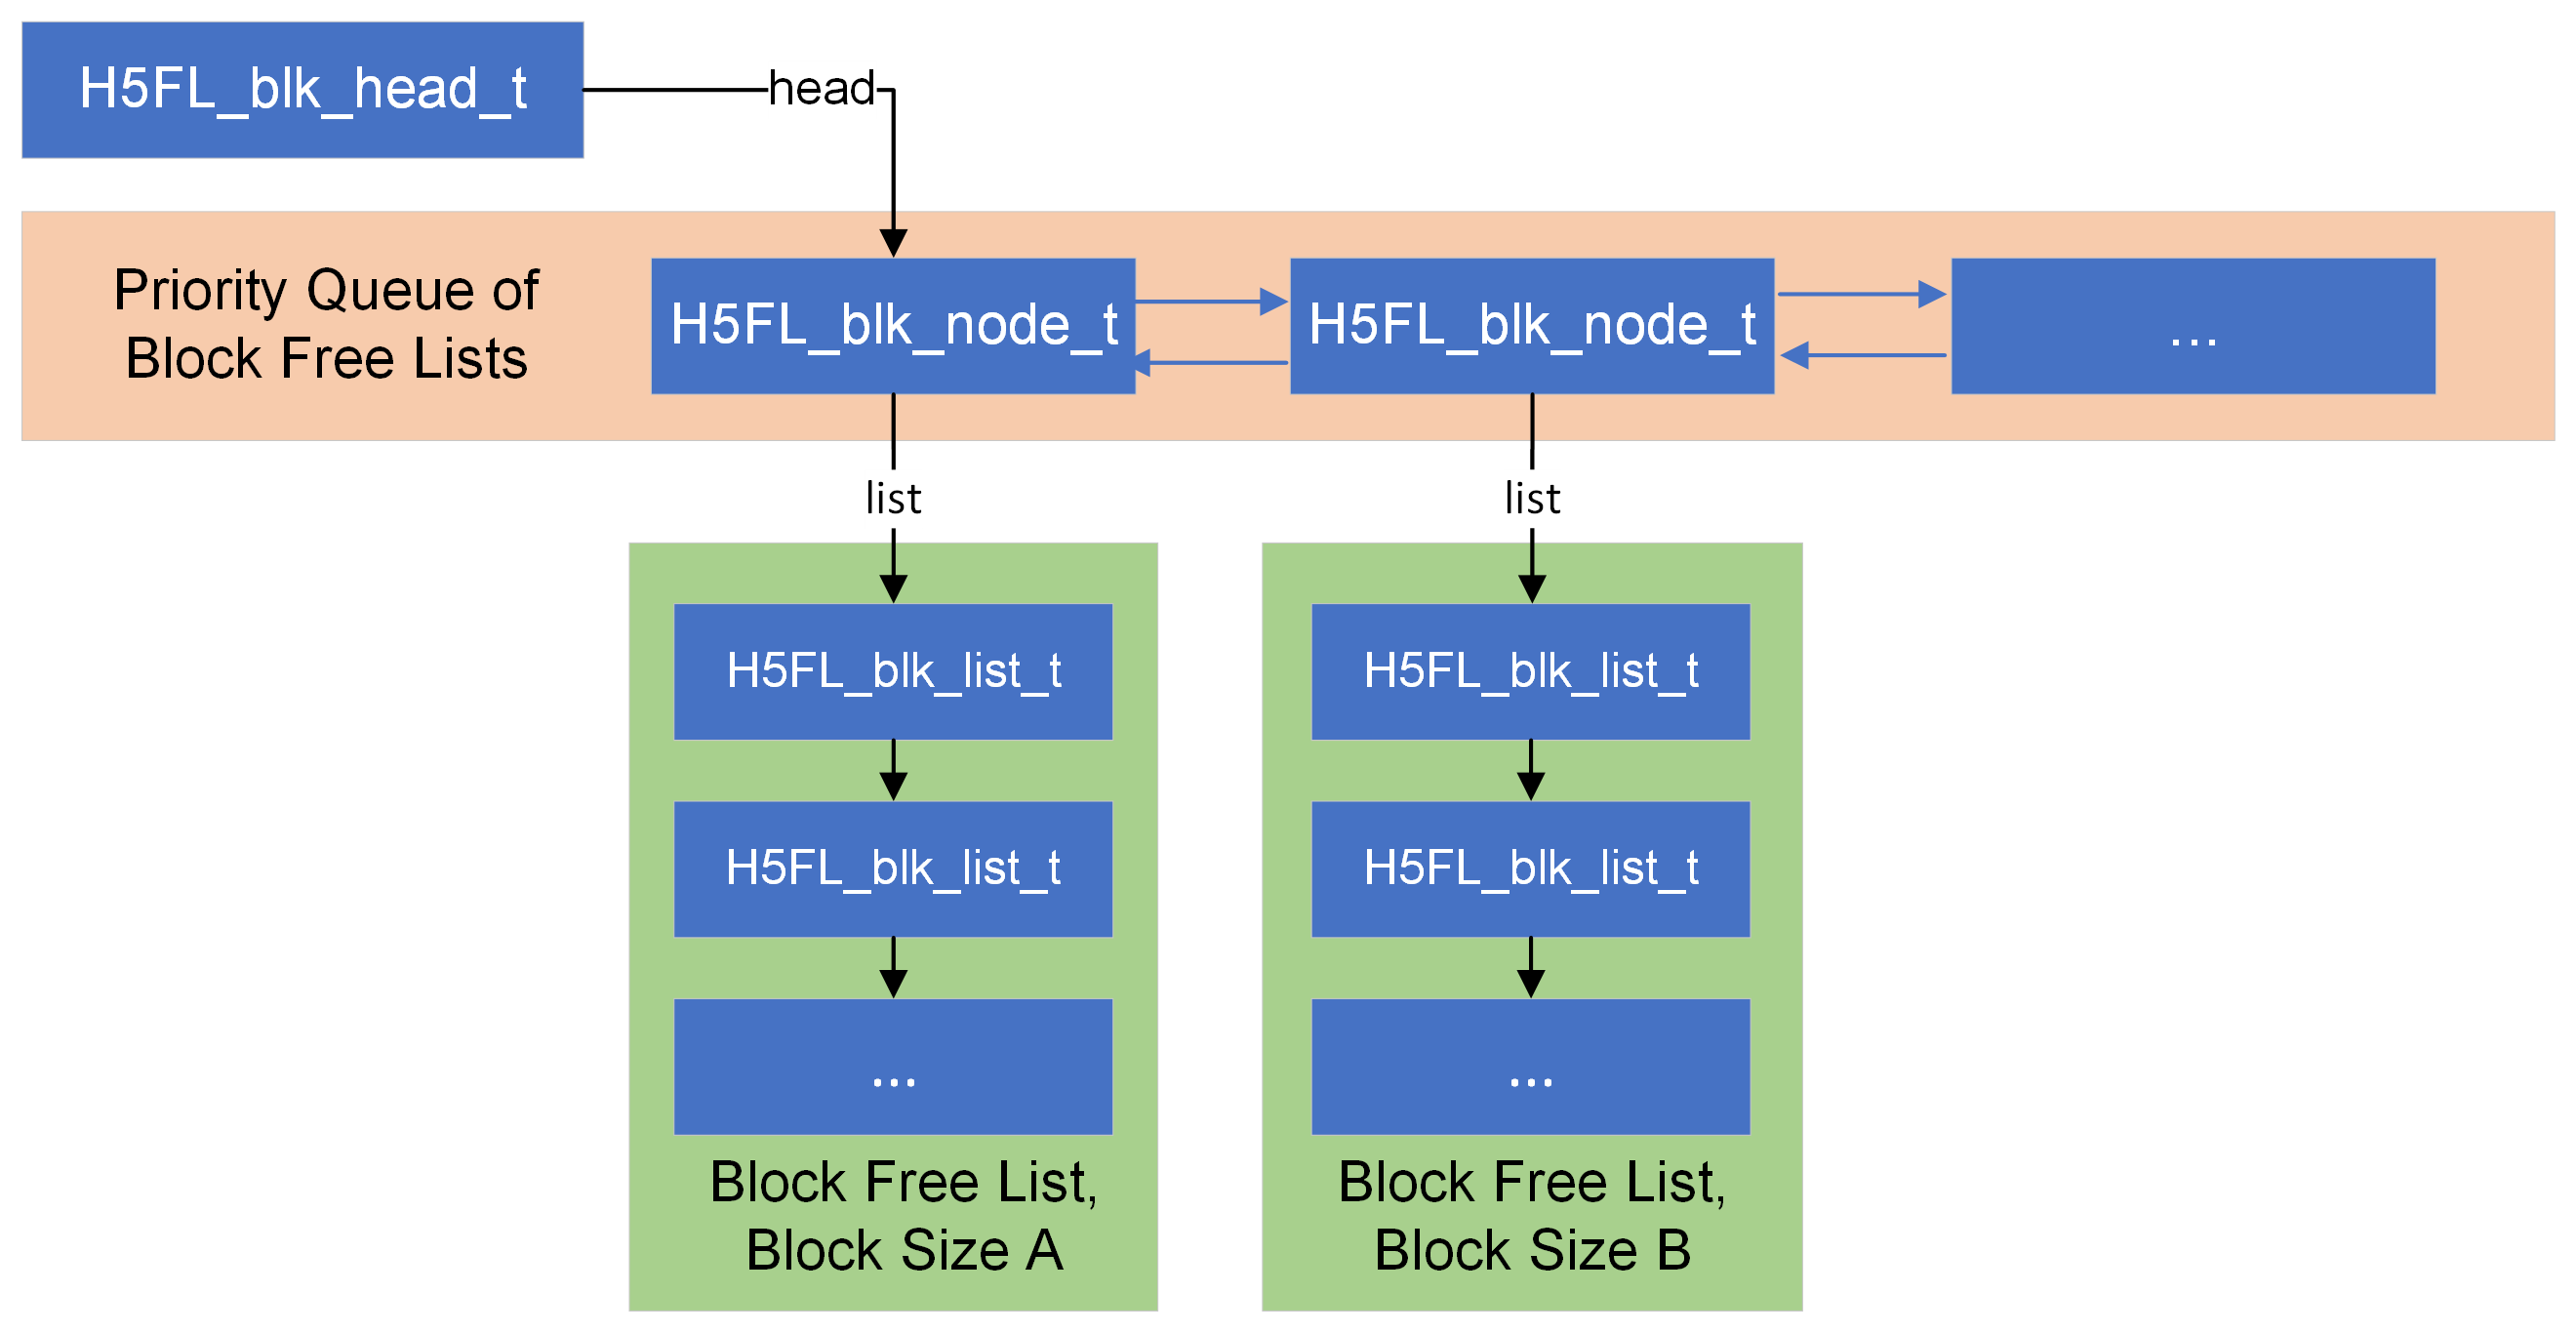
\includegraphics[width=0.8\textwidth]{images/block_free_list_diagram.png}
    \caption{A block free list}
    \label{fig:block-free-list}
\end{figure}

When a memory allocation for a block or array is requested from a free list, the collection of free lists for various block/array sizes is searched for the appropriate free list, and if a free list of the appropriate size is found, a block of memory from that free list is used. In the case of a free block list, the free list that was found is moved from its original position to the head of the queue, speeding up subsequent accesses.

\item Garbage Collection

A major benefit of library-handled free lists is that they enable library-handled garbage collection. Garbage collection is the process by which the library returns library-managed free space to the filesystem.

Garbage collection functionality is exposed to applications through \texttt{H5garbage\_collect}. This is one of many ways that the library exposes the memory and performance tradeoff to applications - less frequent garbage collection will use more memory but involve fewer system calls, while frequent garbage collection keeps memory overhead low but may involve slow allocations.

When a request for memory allocation (through \texttt{H5MM}) cannot be satisfied by the system, the library runs garbage collection and retries the system memory allocation call before throwing an error. This avoids a scenario where the library has memory available to it through free lists, but requests to the system for memory allocation fail due to the system being unaware of this memory.

\item Performance Considerations

Free lists are not created for all library types that require memory allocation. Because the free list infrastructure imposes some overhead in terms of memory and performance, only types that are expected to be allocated and deallocated many times during typical library operation are managed through a free list. Other types have their memory allocated and freed more directly through the \texttt{H5MM} module.

\end{itemize}

\subsection{API Contexts (\texttt{H5CX})}

%|  Name  | TODO | ONGOING | DONE |
%|--------|------|---------|------|
%| Dana   | x    |         |      |
%| Gerd   | x    |         |      |
%| Glenn  | x    |         |      |
%| Jordan | x    |         |      |
%| Luke   | x    |         |      |
%| Matt   |      |         |  x   |
%| Neil   | x    |         |      |
%| Scot   | x    |         |      |

%\todo[inline]{Owner: Matt -- Priority: Medium -- Effort: M -- Completion: 100\%}
\begin{itemize}

\item API Contexts vs. Global Variables

The primary goal of API contexts is to provide a way to get and set values from many different layers of the library during an API routine, without the performance penalty and complexity of extra parameters, and without the tight inter-module coupling and un-traceability of global variables.

To accomplish this goal, each API routine creates an API context containing fields. These fields control aspects of the operation, deciding things such as which VOL to use, or whether a metadata read is collective. Each of the fields in a context is associated with its own accessor ("get/set") routines. At the end of the API routine, the context is released. The temporary lifetime and accessor-based usage of API contexts avoid the shortcomings of global variables, while avoiding the performance penalty of passing around many extra parameters.

\item In-memory objects

An API context is represented by the \texttt{H5CX\_t} struct. This struct has at least one member for each field that is accessible through the API context interface. There are four distinct kinds of context fields, described in Table~\ref{table:H5CX_fields}

\begin{table}[h!]
\begin{tabular}{||c|m{0.70\textwidth}||}
\hline
\textbf{Context Field Type} & \textbf{Description} \\  [0.5ex] 
\hline\hline
Reference Property Lists &  The property lists to use for this operation. May be default or provided by the application. The context stores pointers to the underlying property list objects (\texttt{H5P\_genplist\_t}) without copying them. These fields are used to retrieve property lists for operations that require them in modules such as \texttt{H5FD}. \\
\hline
Internal Fields & Used for managing state that doesn't correspond to a property from a property list. Generally set at a high level and used at a low level. For example, the metadata "tag" is set in high-level group/dataset code and used in the low-level metadata cache. \\
\hline
Cached Fields &  Cached fields correspond to properties from property lists. In general, context fields are retrieved from the underlying property list and saved in the context on-demand. However, if the context contains a default property list, then the context fields are retrieved from cached fields instead. These cached fields are populated from the default property list during library initialization. These cached accesses are faster due to bypassing property list operations. Changes to cached field values do not propagate to the original property lists. \\
\hline
Return-Only Fields & Return-only fields correspond to properties from property lists that are never retrieved within the library and are only set with values in order to return those values to the application. When a value is set in a return-only field, that value is cached in the context until the context is destroyed when the API routine returns. At that time, any return-only fields that have changed have their new values written into the provided property list(s). \\
\hline
\end{tabular}
\caption{API Context Field Types}
\label{table:H5CX_fields}
\end{table}

Cached fields and return-only fields are paired with an additional field \texttt{<field\_name>\_valid}, used by macros that interact with that property. 

\item Reentrancy and The Context Stack 

Some API routines, such as \texttt{H5Literate}, involve user-defined callbacks which may themselves call API routines. Thus, API contexts must be re-entrant safe. This is handled by storing multiple API contexts on a stack, where the topmost context on the stack is used by the most recent API routine in the call stack.

Nodes on the API context stack are represented by the struct \texttt{H5CX\_node\_t}. Each node contains a pointer to an \texttt{H5CX\_t} instance with the actual information for that context, and a pointer to the next (lower) node in the stack. 

Each API call uses the macro \texttt{FUNC\_ENTER\_API} (or \texttt{FUNC\_ENTER\_API\_NOCLEAR}) to initialize and allocate a new context node. This context node is pushed to the top of the context stack by \texttt{H5CX\_push}. The end of each API call uses the macro \texttt{FUNC\_LEAVE\_API} to free the context node and remove it from the context stack with \texttt{H5CX\_pop}.

\texttt{H5CX\_push\_special}/\texttt{H5CX\_pop\_special} are only used in the library termination routine \\ \texttt{H5\_term\_library}. The normal push and pop routines use the library's free-list memory allocation and free routines. During library termination, the free-list and memory management structures are shut down. Thus, to avoid dependency on these structures, the special push and pop functions use system memory calls instead. 

\item API Context Setup

API routines need to use certain functions, depending on their parameters, to set up their API context correctly. The use case and description for each of these functions are in Table~\ref{table:H5CX_functions}.

\begin{table}[h!]
\begin{tabular}{||c|m{0.25\textwidth}|m{0.45\textwidth}||}
\hline
\textbf{Context Function} & \textbf{Use Case}  & \textbf{Description} \\  [0.5ex] 
\hline\hline
\texttt{H5CX\_set\_apl} & Routines with an access property list parameter & Stores the access property list in the context, sets the collective metadata read flag in the context, and enables sanity checks during collective API operations. \\
\hline
\texttt{H5CX\_set\_loc} & Routines that modify file metadata \textbf{without} an access list parameter & Sets the collective metadata read flag in the context, and enables sanity checks during collective API operations. \\
\hline
\texttt{H5CX\_set\_lapl} &  Routines which have both an object-specific access property list, and a link access property list (LAPL) & When a routine takes two access property lists, the object-specific access property list should be set with \texttt{H5CX\_set\_apl}, and the LAPL should be set with \texttt{H5CX\_set\_lapl}. \\
\hline
\texttt{H5CX\_set\_dxpl} &  Routines with a data access property list (DXPL) parameter & Stores the provided DXPL in the context. \\
\hline
\end{tabular}
\caption{API Context Setup Routines}
\label{table:H5CX_functions}
\end{table}

\item Thread Safety and Parallel

Each API context stack is thread-local. As a consequence, API contexts are inherently thread-safe, and API contexts do not require special consideration when using parallel HDF5. Several fields in the context are used to store and retrieve information about collective operations for the MPI-IO VFD, but this procedure is rank-local and entirely adheres to the usage pattern of other context fields.

\end{itemize}

\subsection{Error Handling (\texttt{H5E})}
\todo[inline]{Owner: Matt -- Priority: Low -- Effort: M - Completion: 100\%}

\begin{itemize}

\item Error Messages

An error message is an in-memory object represented by the \texttt{H5E\_msg\_t} struct. An error message contains a string describing the error that occurred, a 'type' indicating whether the error is major or minor, and a pointer to the error class it belongs to. Because error messages contain a dynamically allocated error string, they are reference-counted objects which are assigned handle IDs by the library, and have their own create and close API (\texttt{H5Ecreate\_msg}, \texttt{H5Eclose\_msg}).

\item Error Records

Error records are complete descriptions of individual errors. An error record is implemented as the \texttt{H5E\_error2\_t} struct, which consists of a major error message, a minor error message, an error class, a description of the specific error that occurred, and the location at which the error occurred in the source code. 

\item Error Stacks

An error stack is a collection of error records. By default, when an error occurs in a library function, an error record is pushed onto the active error stack and that function returns a failure indication. Its caller detects the failure, pushes another error record onto the stack, and returns another failure indication. This continues until the API function called by the application returns a failure indication. The library has a default error stack. Generally, errors cause this stack to be printed to the standard error stream automatically. \texttt{H5E\_DEFAULT} may be provided as an error stack ID to indicate the library's default error stack to error API functions. The library's currently active error stack is stored as the globally accessible \texttt{H5E\_stack\_g}. 

An error stack is implemented as an \texttt{H5E\_t} struct. Each error stack is created with space for a fixed amount error records. If more than this amount of errors are pushed onto a single stack, excess error records are truncated, and only the innermost errors will remain.

When an error record is pushed onto an error stack, the information of the record is not copied. Pointers to the record's error class and error messages are stored, and \texttt{H5I\_inc\_ref} increases the reference count of those objects. Correspondingly, when a record is removed from a stack, these pointers are removed and the reference count to the record's fields are decreased via \texttt{H5I\_dec\_ref}.

Most top-level API functions clear the active error stack upon entry, through the \texttt{FUNC\_ENTER\_API} macro, which calls \texttt{H5E\_clear\_stack}. Certain error-handling API functions, such as \texttt{H5Eprint2}, do not clear the error stack, since this would destroy the information they are meant to work with. Error clearing is avoided by replacing the API entry macro with the similar \texttt{FUNC\_ENTER\_API\_NOCLEAR}. Private library functions, which call \texttt{FUNC\_ENTER\_NOAPI} upon entry, and package library functions, which use \texttt{FUNC\_ENTER\_PACKAGE} upon entry, do not clear the error stack.

\item Error Reporting Macros

Error reporting in library functions is usually handled by the macro \texttt{FUNC\_GOTO\_ERROR}. This macro takes a major and minor error code, a return value to indicate failure, and a message. If automatic error reporting is enabled, it uses the preprocessor macros \texttt{\_\_FILE\_\_}, \texttt{\_\_func\_\_}, and \texttt{\_\_LINE\_\_} to add an error to the active error stack with information about the file, function, and line on which the error occurred. Afterwards, it jumps to the \texttt{done} label of the parent function, where cleanup and failure handling are generally performed.

If an error occurs after the \texttt{done} label, use of \texttt{FUNC\_GOTO\_ERROR} could potentially result in an infinite loop. To prevent this, the macro \texttt{FUNC\_DONE\_ERROR} performs the same error reporting without jumping to the \texttt{done} label, and is used whenever an error occurs during function cleanup or error handling.

\item Error Classes

 An error class is a collection of major and minor error messages. Error records must belong to an error class. An application can register a new custom error class with the library via \texttt{H5Eregister\_class}. An error class is implemented as a \texttt{H5E\_cls\_t} struct containing only the three strings provided to \texttt{H5Eregister\_class}, consisting of the error class's name, the library to which the error class belongs, and the version of that library. When using \texttt{H5Eprint2}, the error class of a set of records is displayed as \texttt{<ERROR\_CLASS>-DIAG}. 

\item Customized Error Handling

A user can define their own error reporting callback of type \texttt{H5E\_auto2\_t}. When an API function returns a failure indication, this callback will be invoked on the error stack. The default error reporting callback, \texttt{H5Eprint2}, uses \texttt{H5Ewalk} to traverse the individual error records within an error stack. \texttt{H5Ewalk} invokes a \texttt{H5E\_walk\_t} callback on each error record, and traverses the error stack.

\texttt{H5Eget\_current\_stack} registers the library's current error stack as an in-memory object, and assigns it a handle ID. This clears the active error stack, but leaves the error records that were in the active error stack accessible within the returned error stack object. Once an error stack is assigned a handle, custom error handling can be performed directly through the error API. 
\end{itemize}

% \subsection{Handles \& IDs (\texttt{H5I})}\label{ref:handles}
% \todo[inline]{Owner: ??? -- Priority: Medium -- Effort: M -- Completion: 0\%}

% Rough outline
% \begin{itemize}
%     \item What is an ID?
%         \begin{itemize}
%             \item A library-managed, reference-counted, handle
%             \item ID types
%             \item ID structure
%             \item Library vs. user-defined
%         \end{itemize}
%     \item ID management
%         \begin{itemize}
%             \item Storing and accessing IDs
%             \item Underlying data
%             \begin{itemize}
%                 \item VOL
%                 \item non-VOL
%                 \item Datatypes are a hybrid
%             \end{itemize}
%             \item Accessing the stored data
%             \item Reference counting
%         \end{itemize}
%     \item Example life cycle
%     \item Special considerations
%         \begin{itemize}
%             \item Initialization and shutdown of the H5I package
%             \item Global state and thread-safety considerations
%             \item Future IDs
%             \item Iterating and deletion
%             \item Flushing and ID preservation
%         \end{itemize}
% \end{itemize}

\subsection{Metadata Cache (\texttt{H5[AC,C]})}

%|  Name  | TODO | ONGOING | DONE |
%|--------|------|---------|------|
%| Dana   | x    |         |      |
%| Gerd   | x    |         |      |
%| Glenn  | x    |         |      |
%| Jordan | x    |         |      |
%| Luke   | x    |         |      |
%| Matt   |      |         |  x   |
%| Neil   | x    |         |      |
%| Scot   | x    |         |      |

\todo[inline]{Owner: Glenn -- Priority: High -- Effort: M -- Completion: 60\%}

The metadata cache is a cache meant for speeding up access to HDF5 metadata, and has support for features such as cache size adjustment under automatic or user program control. 

The cache itself is like a very modified version of the UNIX buffer cache, and uses a "Least Recently Used" (LRU) replacement policy to determine which items within the cache get evicted first. Due to the fact that the metadata written to a file can grow without bounds, the size of the metadata cache must reflect this ability, and no max entry amount can be set. Instead, users may set a maximum size, and eviction will occur as necessary using the LRU replacement policy. Similarly to UNIX, when dirty entries reach the end of the cache, they are flushed, marked as clean, and reset to the beginning of the cache. When running in parallel, only process 0 is allowed to write metadata to the file, and it does so only at synchronization points.

It is possible to tell when the size of the cache is a problem and must increase based on the hit rate, which is calculated over a period of time known as an epoch. When the hit rate has been low for a while, it means that the cache is probably at maximum capacity, and its capacity is probably not big enough. If this is the case, the size will increase according to some user-defined multiple. 

In addition, if the metadata entry is larger than the cache itself, this could also cause problems. This issue is fixed whenever it appears by taking the size of the metadata entry, multiplying it by some preset factor, and increasing the size of the cache based on this new size. 

Both of the above problems may arise when cache sizes are too big. Similarly, issues can occur when the cache size is too small. However, this is harder to judge. Ageout with hit rate threshold is the default cache size reduction algorithm of choice, and it combines two methods of detecting an oversized cache size. The first involves checking the hit rate once again. If the hit rate exceeds some preset amount, it might mean that the cache size is too big and needs to be reduced. Then, the second part of the algorithm, checking for metadata entries that haven't been accessed in some amount of epochs, kicks in and removes aged out entries. 

The metadata cache's configuration information is stored in a \texttt{H5AC\_cache\_config\_t} struct. This struct contains fields for general information, size increase control fields, size decrease control fields, and parallel configuration fields. 

\subsection{Files and the Open File List (\texttt{H5F})}

%|  Name  | TODO | ONGOING | DONE |
%|--------|------|---------|------|
%| Dana   | x    |         |      |
%| Gerd   | x    |         |      |
%| Glenn  | x    |         |      |
%| Jordan | x    |         |      |
%| Luke   | x    |         |      |
%| Matt   |      |         |  x   |
%| Neil   | x    |         |      |
%| Scot   | x    |         |      |

%\todo[inline]{Owner: Matt -- Priority: High -- Effort: L - Completion: 100\%}

\begin{itemize}
    \item File in-memory objects

Each successful \texttt{H5Fopen} results in a top-level file descriptor \texttt{H5F\_t}. By contrast, \texttt{H5F\_shared\_t}, the underlying structure storing information about the opened file, is allocated only once for each file in storage and is shared between file descriptors that point at the same file. Most of the fields in \texttt{H5F\_shared\_t} represent information related to persisting HDF5 files in a file system according to the file format specification~\cite{ffmt}. The shared file also tracks how many file descriptors point to it, and is only closed when its last file descriptor is closed.

The shared file contains a list of all opened objects, while each file descriptor maintains only counts of how many times each object is opened through that particular file descriptor. This division of information ensures that closing a file descriptor only decrements references that originated through that descriptor. For similar reasons, each file descriptor tracks the total number of objects it has open, excluding the root group.

Most information about child files mounted onto a parent file is kept in a table on the shared file structure of the parent file. The file descriptor maintains only a count of how many files were mounted through itself, similar to its count for open objects. The number of mounted files is maintained so that a file descriptor will close when 1. a weak close (see the section 'File open and close') was previously performed on it, and 2. an object is closed, and the only open objects remaining on the file descriptor are mounted groups. 

The shared file also contains information necessary for I/O, such as the file's permissions in storage, a page buffer, and any free space managers.

 \item Open file list

The file module maintains a list of open shared file objects, \texttt{H5F\_sfile\_head\_g}. Newly opened files are appended to the head of this list. This list is searched when checking if a file is already open. The actual comparison to determine if a potentially non-open file matches an open file is handled by the active VFD, which is not required to provide a way to compare files. If it does not provide such a method, then the application opening multiple handles to the same file will result in undefined behavior, and it is the responsibility of the application to ensure that the same file is not opened multiple times.

The open file list is implemented as a linked list. Due to the need to search this list upon each file open, performance may degrade if there is a large number of open files. The library is optimized for a small number of top-level files that contain many groups and objects in their internal file hierarchy.

    \item File open and close

File opening is first attempted without creating or truncating any files. This allows attempts to truncate or re-create currently opened files to safely fail without modifying any state. If the file is not already open, then the open proceeds normally, modifying files as requested, and the resulting shared file object is added to the open file list.

Each FAPL has a 'file close degree' which determines how open objects within a file are handled at file close. The 'weak' close degree allows the file handle to be closed from the application's perspective (as tracked by the \texttt{closed} flag on a file descriptor), but keeps the file handle around until all objects under it are closed. The root group and the root groups of any mounted files are not considered open objects for this purpose, and a weak close will be completed if such groups are the only open objects remaining. The 'semi' close degree causes a file close to fail if any objects remain open. The 'strong' close degree causes any open objects to be closed before the close completes. Most VFDs default to 'weak', except for the MPI-I/O driver which defaults to 'semi', due to file closes being a collective operation. When HDF5 files are mounted, the parent and child files must have the same close degree in order to avoid contradictions in how to handle objects at close time.

Closing an object may or may not evict it from the file's metadata cache, depending on the 'evict on close' setting. This setting trades increased memory with a larger cache for higher speed, or lower speed with a smaller cache for decreased memory usage.

    \item External file cache

The external file cache (EFC) is a mechanism for keeping files opened through external links quickly accessible for subsequent accesses. Each shared file structure may have an EFC that stores information about files accessed through external links in that shared file.

EFC entries are linked to the top-level file descriptor, as the EFC caches the result of opening an external file (a top-level file descriptor). Because file descriptors are not reference counted, EFC entries must be reference counted within the EFC in order to handle dependencies in the EFC tree.

A file's EFC contains both a skip list of cache entries and the head of a cache entry list sorted by the least recent update (LRU) time. The skip list is used to check whether a newly opened external file is already present in the cache. The LRU-sorted list speeds up the common case of closing the most recently opened external file and allows the least-recently accessed cache entry to be dropped when the maximum size of the EFC is reached.

\end{itemize}

% \subsection{File Space Management and Free Space Tracking (\texttt{H5FS})}
% \todo[inline]{Owner: ??? -- Priority: Medium -- Effort: M -- Completion: 0\%}

\subsection{File Page Buffer (\texttt{H5PB})}\label{sec:H5PB}

%|  Name  | TODO | ONGOING | DONE |
%|--------|------|---------|------|
%| Dana   | x    |         |      |
%| Gerd   | x    |         |      |
%| Glenn  | x    |         |      |
%| Jordan | x    |         |      |
%| Luke   | x    |         |      |
%| Matt   |      |         |   x  |
%| Neil   | x    |         |      |
%| Scot   | x    |         |      |

%\todo[inline]{Owner: Matt -- Priority: High -- Effort: M -- Completion: 100\%}

The page buffer exists within the native VOL, just above the VFL and just below the I/O layer. Thus, the library can benefit from the page buffer cache regardless of which VFD is active. 

There are a few conditions under which file I/O bypasses the page buffer entirely: if page buffering is disabled, if the requested I/O operation is larger than one page and thus would not benefit from the page buffer, or if the requested operation is a parallel raw data access. Additionally, when opening a file with page buffering enabled, the superblock contains information needed to initialize the page buffer (e.g. page size). Because this information must be read from the superblock before the page buffer is initialized, the page buffer cannot be used for this operation.

The page buffer's page size will be rounded down to the nearest multiple of the file space page size, in order to avoid situations where reading or writing in blocks of page size could extend outside the bounds of the file.

\begin{itemize}

    \item In-memory objects

A page buffer is represented in memory by the struct \texttt{H5PB\_t}, which is attached to a shared file object. Page buffers are associated with the shared file so that different handles to the same file share the same page buffer.

The page buffer maintains three lists of pages. The first is a skip list of page entries allocated by the page buffer itself. The second is another skip list containing only the page entries inserted by the free space manager. The free space manager inserts blank pages into this list during reads of file regions that have never been written to, in order to avoid unnecessary file accesses. The third list is a linked list of page entries sorted by the least recent update (LRU). The LRU-sorted list is used to evict the oldest page entries when the maximum size of the page buffer is reached. 

Page buffer entries (\texttt{H5PB\_entry\_t}) consist of their location in the file, pointers used to maintain the LRU-list, and an indication of whether the page buffer entry contains metadata or raw data. 

    \item Metadata vs Raw Data

I/O operations accessing a metadata entry are always atomic - the entire entry is always accessed. Noncontiguous subsets of raw data may be accessed using selections, and so I/O operations on raw data through the page buffer require some additional steps. During raw data writes, the page buffer needs to update any pages that are partially modified by large (greater than page size) writes, and discard any pages that are entirely overwritten. Similarly, during raw data reads, the page buffer must collect data from any dirty pages that are within the span of the I/O request. 

The utility of storing metadata versus raw data in the cache will vary from use case to use case. To allow applications to optimize for their particular case, and to avoid a scenario where one type of data is completely evicted from the page buffer cache, applications may set a minimum percentage of the page buffer's memory to be reserved for each type of data.

A page in the page buffer must contain only metadata or only raw data. This restriction is imposed in order to properly map pages to regions of the file in storage, as metadata and raw data are not interleaved within pages in storage (with the default driver).

    \item Page Buffering in Parallel

Parallel HDF5 has limited support for the page buffer due to the need for all processes to have a mutually consistent view of the data.

Because all operations that modify metadata must be performed collectively, the page buffer can be used during parallel metadata I/O if the metadata write strategy has a single process handle all writing of dirty metadata from cache. This is accomplished by having the writer-process write all dirty entries to the page buffer, flush the page buffer to storage, and then update the other ranks with the metadata entries that were written.

The page buffer is always bypassed when reading or writing raw data in parallel. When accessing raw data collectively, the HDF5 library constructs MPI-derived datatypes to represent possibly non-contiguous buffers in memory and file offsets. At the page buffer layer, it would be necessary to flatten the derived datatypes, update the page buffers, and then impose additional communication among all processes to determine who reads/writes which pages for the collective operation. This would represent considerable overhead and complexity, and replicate work that is more logically handled by MPI itself. Simply bypassing the page buffer likely leads to better performance than this implementation would. Additionally, most parallel raw data accesses are large enough that the page buffer would not provide a significant benefit. While many of these issues would not apply to parallel independent raw data access, concurrent use of collective and independent operations would cause the page buffers of the processes involved in each operation to become inconsistent with one another, and thus the page buffer is bypassed during all parallel operations regardless of whether they are collective or independent.

When using Single Writer Multiple Reader (SWMR), the writer may not make use of a page buffer. The SWMR writer has a required order for its operations, which would not be preserved by the page buffer. SWMR readers can use the page buffer with only one caveat. After a refresh operation is performed on an object, entries that get evicted from the metadata cache must have their corresponding pages evicted from the page buffer in order to avoid subsequent reads returning old data. 

\end{itemize}

\begin{comment}
\subsection{Virtual File Layer (\texttt{H5FD})}\label{ref:vfl}

%|  Name  | TODO | ONGOING | DONE |
%|--------|------|---------|------|
%| Dana   | x    |         |      |
%| Gerd   | x    |         |      |
%| Glenn  | x    |         |      |
%| Jordan | x    |         |      |
%| Luke   | x    |         |      |
%| Matt   | x    |         |      |
%| Neil   | x    |         |      |
%| Scot   | x    |         |      |

\todo[inline]{Owner: Luke -- Priority: Medium -- Effort: S -- Completion: 0\%}

The Virtual File Layer (VFL) provides the ability to extend the native VOL to support I/O to different I/O backends. The purpose of the VFL is to decouple the file I/O functionality from the core HDF5 library, allowing for greater flexibility in supporting different storage mechanisms and file systems. It serves as a "plug-in" layer that allows HDF5 to work with various storage backends.



% \subsection{On-Disk Indexes (\texttt{H5[B,B2,EA,FA]})}
% \todo[inline]{Owner: ??? -- Priority: Low -- Effort: M}

% \begin{itemize}
%     \item v1 B-trees
%     \item v2 B-trees
%     \item Fixed arrays
%     \item Extensible arrays
% \end{itemize}

% \subsection{On-Disk Heaps (\texttt{H5H[F,G,L]})}
% \todo[inline]{Owner: ??? -- Priority: Low -- Effort: M}

% \begin{itemize}
%     \item Local heaps
%     \item Global heaps
%     \item Fractal heaps
% \end{itemize}
\end{comment}

\subsection{File Objects (\texttt{H5[O,SM]})}

%|  Name  | TODO | ONGOING | DONE |
%|--------|------|---------|------|
%| Dana   | x    |         |      |
%| Gerd   | x    |         |      |
%| Glenn  | x    |         |      |
%| Jordan | x    |         |      |
%| Luke   | x    |         |      |
%| Matt   |      |         |   x  |
%| Neil   | x    |         |      |
%| Scot   | x    |         |      |

\todo[inline]{Owner: Neil -- Priority: High -- Effort: L -- Completion: 30\%}

File objects are the heart of the HDF5 data model. In the library, the object package (\texttt{H5O}) consists of structures and code common to all object types, as we use code to handle object headers, which are the central on-disk objects for storing HDF5 file objects. All objects contain an object header, which contains some fixed metadata and a variable list of object header messages, as well as any data referenced by those object header messages.

\begin{itemize}
    \item In-memory objects

The central in-memory structure for an object is \texttt{H5O\_t}, which is defined in \texttt{H5Opkg.h}. This structure essentially contains the information that is stored in the object header, including the list of object header messages. While it might seem natural for the type-specific object structs (such as \texttt{H5D\_t} for datasets) to contain an \texttt{H5O\_t} at the top (beginning) of the struct, this is not the case. \texttt{H5O\_t} is essentially a lower-level proxy for the object header on disk, while the type specific structures are closely tied to the logical objects exposed through the API.

One potential point of confusion is the \texttt{rc} field in the \texttt{H5O\_t} struct is not the same as the \texttt{rc} field in the struct returned by \texttt{H5Oget\_info()}. The \texttt{rc} in \texttt{H5O\_t} is the in-memory reference count of the memory struct itself, while the \texttt{rc} returned by \texttt{H5Oget\_info()} is the number of links to the object header in the file. The \texttt{nlinks} field in \texttt{H5O\_t} is equivalent to the link-counting \texttt{rc} from \texttt{H5Oget\_info()}.

    \item Object headers

The object header is the root piece of metadata for all HDF5 objects on disk. The object header consists of the main object header block, which in turn consists of the prefix containing generic object metadata, as well as some number of object header messages. If the number of messages grows too large to fit into the main object header block, one or more object header continuation chunks will be created on disk, each containing more object header messages. Object header continuation blocks are pointed to from their parent object header using an object header continuation message.

Since an object header is not a single block on disk, but is treated as a single object by most of the library, the way the metadata cache handles it is slightly strange. There are metadata cache clients for object header root blocks and continuation blocks, each of which serializes and deserializes these objects as needed. However, when the entire object header is retrieved, typically using \texttt{H5O\_protect()} or \texttt{H5O\_pin()}, which take an \texttt{H5O\_loc\_t} object location, these functions use the metadata cache to decode all the constituent blocks of the object header, protects (and optionally pins) the root object header block, then assembles and returns an \texttt{H5O\_t}. The \texttt{H5O\_loc\_t} struct is how other packages generally keep track of their objects and mostly consists only of a file and address of the root object header block.

    \item Object header messages

Object header messages encode the majority of the important metadata of the object. There are several different types of object header messages, and only some of them are present in any one object header. The type of an object is determined by which object header messages are present. For example, if a layout message is present, then the object is a dataset. Object header messages also appear in the file superblock, even though that is not an object header.

Each object header message type is defined in a separate source file, for example, \texttt{H5Olayout.c} for layout messages. Each message type defines itself using the \texttt{H5O\_msg\_class\_t} struct, which contains callback functions that must be implemented (some are optional) and other basic information about the message type. Most object header message types can only be present once in an object header, but there are some exceptions, such as attributes, link messages, and object header continuation messages. This distinction is important since \texttt{H5O\_msg\_read()} only reads the first message of a given type, so if there may be more than one message of that type, \texttt{H5O\_msg\_iterate()} must be used instead, with the callback operation checking to see if it is the correct message. The generic (type agnostic) object header message code stores messages in the \texttt{H5O\_mesg\_t} struct. This struct contains information on allocation within the object header, as well as pointers to the serialized/on-disk form (\texttt{raw}) and the deserialized/in-memory form (\texttt{native}). The in-memory structs for all the different message types are defined in \texttt{H5Oprivate.h}. They are defined in the private header because other packages widely use the native forms of these messages. This makes \texttt{H5Oprivate.h} one of the most important header files in HDF5, and can be thought of as a significant contributor to the coupling between the packages.

Allocation of space for object header messages is somewhat complicated and handled in \texttt{H5Oalloc.c}. This code handles allocation, deletion, free space tracking (with null messages), and the creation of new continuation blocks (in conjunction with the metadata cache and standard file space allocation code). This code needs to handle several corner cases, such as when a message is added when there isn't enough space for a continuation message (in this case it must move messages), or if there's empty space but there isn't space for a null message (in this case it encodes a "gap" value in the object header).

    \item Shared object header messages

To save space, the HDF5 library can optionally automatically check if object header messages are the same between different objects, and only store this message once if that is the case. Such messages are called shared object header messages, and can be stored either in one object's object header, or in the file's shared object header message heap. Additionally, these shared messages can be indexed either with a simple list or a v2 b-tree. Using a v2 b-tree obviously improves the performance of checking to see if a message is already shared, but requires a more recent file format version.

Object header messages that can be shared need to follow special steps in their definition files. First, they need to \texttt{\#include H5Oshared.h}, then, for the callbacks which are defined in \texttt{H5Oshared.h}, they need to \texttt{\#define} the callback from \texttt{H5Oshared.h} to a name specific to the message type (this name isn't actually defined in the message file, it's used to point to the shared function from the header), then do the same with the symbol that ends in \texttt{\_REAL}, defining it to be the name of the actual function implemented in the object header message definition file. For example, \texttt{H5Odtype.c} uses: \texttt{\#define H5O\_SHARED\_DECODE H5O\_\_dtype\_shared\_decode}, where \texttt{H5O\_\_dtype\_shared\_decode} is only used as the name for the \texttt{decode} callback in the \texttt{H5O\_msg\_class\_t} struct; \texttt{\#define H5O\_SHARED\_DECODE\_REAL H5O\_\_dtype\_decode}, where \texttt{H5O\_\_dtype\_decode()} is defined as the actual datatype decoding function in \texttt{H5Odtype.c}, which does not handle shared messages. Therefore, when the library decodes a datatype message, the code flows into \texttt{H5O\_SHARED\_DECODE()}, which locates the actual datatype message and then invokes \texttt{H5O\_\_dtype\_decode()} to do the actual decoding.

For callbacks that are not implemented by the object header message definition file, they must still \texttt{\#define} the callback from \texttt{H5Oshared.h} to a name and include that name in the class struct, but they may then \texttt{\#undef} the \texttt{\_REAL} version of the callback. In addition, the object header message definition file must \texttt{\#define H5O\_SHARED\_TYPE} to the name of the global variable containing its \texttt{H5O\_msg\_class\_t} class struct.

Additional code for handling shared messages in these callbacks is defined in \texttt{H5Oshared.c}, while most of the code for handling shared messages (allocation, search, etc.) is contained in the \texttt{SM} package. Code for handling the message in the file superblock which points to the shared message heap is contained in \texttt{H5Oshmesg.c}.

    %\item Object copying

%\todo[inline]{Object copying}

\end{itemize}

\subsection{Attributes (\texttt{H5A})}

%|  Name  | TODO | ONGOING | DONE |
%|--------|------|---------|------|
%| Dana   | x    |         |      |
%| Gerd   | x    |         |      |
%| Glenn  | x    |         |      |
%| Jordan | x    |         |      |
%| Luke   | x    |         |      |
%| Matt   |      |         |  x   |
%| Neil   | x    |         |      |
%| Scot   | x    |         |      |

%\todo[inline]{Owner: Matt -- Priority: High -- Effort: M -- Completion: 100\%}

\begin{itemize}
    \item Attribute in-memory objects

Attribute in-memory objects are represented with the \texttt{H5A\_t} structure, defined in \texttt{H5Apkg.h}. This structure contains information about whether the attribute is shared between multiple objects, the location of the attribute's parent object on disk, and the path to the attribute in the file hierarchy. The underlying shared attribute object \texttt{H5A\_shared\_t} contains information such as the size of the attribute, its dataspace and datatype, and its name. The shared \texttt{nrefs} field tracks the number of remaining references to the attribute from other objects in the file, and the attribute's resources are freed once this count is decremented to zero. 

The \texttt{crt\_idx} field tracks the creation index of the attribute, if creation index tracking is enabled on the parent object. This index only tracks the order in which attributes were created relative to each other, not any absolute information about the time of their creation.

    \item Compact and Dense Attribute Storage

There are two kinds of attribute storage: compact and dense. Compact attributes are kept in the object header of the parent object, along with other metadata for that object. Dense attributes are kept in a fractal heap. The address of the fractal heap for dense attribute storage is kept in the Attribute Info message in the object header. The heap IDs to access specific dense attributes in the fractal heap are stored in a name-index B-tree. 

If the file access property list used for a file is set for file format compatibility with library versions before 1.8 (as is the case by default), all attributes will be stored compactly, and the creation of attributes larger than 64 KiB will not be allowed.

The architecture for attribute storage is nearly identical to the architecture for link storage.

    \item Attribute object header messages (open/flush)

The primary fields that define an attribute are its datatype, dataspace, name, and the data it contains. When an attribute is compact, all of these fields are stored in an attribute object header message and inserted into the object header of the parent object. In library file format versions 1.6 and later, the datatype/dataspace fields in an attribute message may be pointers to a datatype or dataspace message that is shared between objects.

If an object is using dense attribute storage, then the object header will contain an attribute info message with the location of a name-index B-tree, as well as the address of the fractal heap storing the attribute messages.

Changes to object headers make use of caching for optimization. Attribute messages may be flushed to storage by use of \texttt{H5Fflush} on the containing file, or \texttt{H5(D/G/T/O)flush} on an object of the appropriate type with attached attributes. Note that these functions only directly control the library's buffers, not any buffering performed by the operating system. Flushing of object headers is also performed automatically by the library during certain operations.

    \item Attribute I/O

Attributes do not support partial reads or writes using selections. Any read or write to an attribute will operate on the attribute's entire dataspace. Attributes also do not support compression or chunking. Because attributes are intended to hold small quantities of metadata, these aspects of the I/O pipeline were omitted in order to optimize and simplify attribute I/O. If any of these I/O features are desired for use with metadata, then that metadata may be stored in a dataset instead, and a pointer to that dataset stored in an attribute - see the section "Dataset Storage Layouts".

Reads and writes to attributes use the same datatype conversion pipeline as read and writes to datasets.

If an attribute in compact storage is written to, all of its previous data in the object header is overwritten by an in-memory buffer that is later flushed to storage. If an attribute in dense storage is written to, a write operation is performed on the fractal heap at the heap ID storing the attribute by name. 

    \item Attribute iteration

The iteration process varies between compact and dense attributes.

Dense attribute iteration is handled by \texttt{H5A\_\_dense\_iterate}. If the iteration order was specified to be \texttt{H5\_ITER\_NATIVE} in order to optimize for speed, then the order is determined by the hashes of the attribute names in the name index B-tree. Otherwise, a table of attributes is built by \texttt{H5A\_\_dense\_build\_table}, sorted in the desired order by \texttt{H5A\_\_attr\_sort\_table}, and then iterated through by \texttt{H5A\_\_attr\_iterate\_table}.

The compact iteration case is similar: \texttt{H5A\_\_compact\_build\_table} creates a table of attributes, and iterates through it via \texttt{H5A\_\_attr\_iterate\_table}. For compact attributes, the table is always constructed, even when the iteration order is \texttt{H5\_ITER\_NATIVE}. 

The attribute table itself is the same, regardless of the storage type its attributes were retrieved from.

The architecture for attribute iteration is nearly identical to the architecture for link iteration. As with all forms of iteration in the library, attributes should not be created or removed during iteration - changes to the parent object's attribute count during iteration can lead to undefined behavior.

\end{itemize}

\subsection{Groups and Links (\texttt{H5[G,L]})}

%|  Name  | TODO | ONGOING | DONE |
%|--------|------|---------|------|
%| Dana   | x    |         |      |
%| Gerd   | x    |         |      |
%| Glenn  | x    |         |      |
%| Jordan | x    |         |      |
%| Luke   | x    |         |      |
%| Matt   |      |         |  x   |
%| Neil   | x    |         |      |
%| Scot   | x    |         |      |

%\todo[inline]{Owner: Matt -- Priority: High -- Effort: L -- Completion: 100\%}

A group is a potentially empty collection of link objects. The name of an object within a group is actually the name of a link that refers to it. The same underlying object may be referred to by multiple names, if it is pointed to by multiple links in one or more groups. When an object is created by a user, the library automatically creates a new hard link from the parent group to that object.

\begin{itemize}

    \item Group in-memory objects

Groups are represented by the \texttt{H5G\_t} struct. This struct has three elements: the location of the group within the file hierarchy as an \texttt{H5G\_name\_t} instance, the group's address within the file as an \texttt{H5O\_loc\_t} instance, and shared information for the group as an \texttt{H5G\_shared\_t} instance. The shared group information is available to all in-memory objects which refer to the same underlying group in the file, and allows a shared count of how many in-memory objects reference that particular group to be maintained. % This count is used to manage when the metadata cache is flushed. The metadata cache is flushed when the number of group in-memory objects for a particular group drops to zero (i.e. the last reference to that group is closed).

    \item Link storage

There are two kinds of link storage: compact and dense. Compactly stored links are kept in the object header for the group containing them, along with other metadata for that group object. Densely stored links are kept in a fractal heap. The address of the dense link fractal heap is then stored in the Link Info message in the group's header, with the heap IDs to access specific dense links stored in the name index B-tree. 

If the file access property list used for a file is set for file format compatibility with library versions before 1.8 (as is the case by default), all links will be stored in the file's symbol table.

% If compact storage is used, the link message is inserted into the header of the target group by \texttt{H5G\_\_compact\_insert}. The object header is pinned while the new message is appended, preventing it from being flushed to file, and unpinned after the operation is finished. When a compact link is accessed by name, the search is performed by \texttt{H5G\_\_compact\_lookup}, which iterates over the messages in the group header with \texttt{H5O\_msg\_iterate} and uses \texttt{H5G\_\_compact\_lookup\_cb} to check for a match by link name and copy the message if a match was found.

% If dense storage is used, the insertion of of the link is handled by \texttt{H5G\_\_dense\_insert}, which in turn uses \texttt{H5HF\_insert} to insert link information into the dense link fractal heap and \texttt{H5B2\_insert} to insert the link's name (and potentially, its creation order) into a v2 B-tree. Accessing dense links is handled by \texttt{H5G\_\_dense\_lookup}, which uses \texttt{H5B2\_find} to search the name index v2 B-tree for a dense link with the target name. If the dense link is found, then the provided callback \texttt{H5G\_\_dense\_lookup\_cb} copies the link message information.

The architecture for dense/compact link storage is nearly identical to the architecture for attribute storage.

    \item User-defined links

Users may register a user-defined link class with \texttt{H5Lregister}, and then create a link of that class using \texttt{H5Lcreate\_ud}. A link class definition must at minimum include a version number for the link class struct \texttt{H5L\_class\_t}, a link class identifier \texttt{class\_id}, and a traversal function \texttt{trav\_func}. \texttt{link\_class} must be in the range between \texttt{H5L\_TYPE\_UD\_MIN} and \texttt{H5L\_TYPE\_UD\_MAX}. Note that external links are implemented as an example of a user-defined link class, using \texttt{class\_id} = \texttt{H5L\_TYPE\_UD\_MIN}.

User-defined link classes may also provide optional callback functions to create, move, copy, delete, and query an instance of the link class. Some functionality is automatically implemented for these callbacks as a consequence of the type-independent link architecture. 

Depending on the user's implementation of the link callbacks, user-defined links may or may not affect the \texttt{nlinks} count of objects, and may or may not be allowed to dangle.

    \item Link traversal

"Link traversal" refers to the process of following links to their target objects. When opening an object through a link, the link's target location in the file hierarchy is iteratively determined by \texttt{H5G\_traverse}, and once the target location is reached, location information specifying position within the file hierarchy (\texttt{H5G\_name\_t}) and within the file (\texttt{H5O\_loc\_t}) is copied to the opened object.

For hard links, if the hard link points to a mounted file, then \texttt{H5F\_traverse\_mount} performs a binary search over the mount table of the original file in order to copy the root group location information of the mounted file. 

For soft links, traversal of the target path is performed by \texttt{H5G\_\_traverse\_slink}. The file hierarchy traversal process of \texttt{H5G\_traverse} is repeated on the path specified by the soft link. Because soft links are allowed to dangle, this traversal may find that no object exists at the target location, or that the object is of an unexpected type.

For user-defined links, the provided traversal callback is invoked in \texttt{H5G\_\_traverse\_ud}. 

For external links, the traverse callback \texttt{H5L\_\_extern\_traverse} handles opening the external file and locating the target object within it.

    \item Link iteration

Iteration over all links in a group may be performed through \texttt{H5Literate} non-recursively, or \texttt{H5Lvisit} recursively. \texttt{H5Literate}, when using the native VOL, passes control to \texttt{H5L\_iterate}, which internally uses \texttt{H5G\_iterate}. Similarly, \texttt{H5Lvisit} ultimately passes control to \texttt{H5G\_visit}. Making the relationship between groups and links clear was one of the reasons that the iteration functions in the \texttt{H5G} module were deprecated in favor of \texttt{H5Lvisit/iterate}. 

The iteration process varies based on whether the group is currently using dense or compact storage (or a symbol table, for old versions of the file format). 

Dense link iteration is handled by \texttt{H5G\_\_dense\_iterate}. If the iteration order was specified to be \texttt{H5\_ITER\_NATIVE} in order to optimize for speed, then the order of link iteration is determined by the hashes of the link names in the name index B-tree. Otherwise, a table of links is built by \texttt{H5G\_\_dense\_build\_table}, sorted in the desired order by \texttt{H5G\_\_link\_sort\_table}, and then the link table is iterated through by \texttt{H5G\_\_link\_iterate\_table}. % The table is implemented as an array of pointers to link objects (\texttt{H5O\_link\_t}) that keeps track of its total length.

The compact iteration case is similar: \texttt{H5G\_\_compact\_iterate} uses \\ \texttt{H5G\_\_compact\_build\_table} to create a table of links and iterates through it via \\ \texttt{H5G\_\_link\_iterate\_table}. For compact links, the link table is always constructed, even when the iteration order is \texttt{H5\_ITER\_NATIVE}. 

The link table itself is the same, regardless of the storage type its links were retrieved from.

The architecture for attribute iteration is nearly identical to the architecture for link iteration.

\end{itemize}

\subsection{Datasets (\texttt{H5D})}

%|  Name  | TODO | ONGOING | DONE |
%|--------|------|---------|------|
%| Dana   | x    |         |      |
%| Gerd   | x    |         |      |
%| Glenn  | x    |         |      |
%| Jordan | x    |         |      |
%| Luke   | x    |         |      |
%| Matt   |      |         |  x   |
%| Neil   | x    |         |      |
%| Scot   | x    |         |      |

\todo[inline]{Owner: Neil -- Priority: High -- Effort: L -- Completion: 100\%}

\begin{itemize}
    \item Dataset objects

A dataset is an HDF5 object which stores raw array data. Each dataset must include layout, dataspace, and datatype object header messages, and may optionally include pipeline, fill value, and EFL (external file list) messages, in addition to generic messages like attributes and modification time. The layout message stores information about how the data is laid out in the file, for example, the location of the address for the chunk index, the location of the contiguous data block, or the actual data for compact datasets. The dataspace message contains the extent (dimensions) of the dataset. The datatype message contains a description of the format of a single element of data in the dataset as stored in the file.

    \item Dataset in-memory objects

Like other HDF5 objects, a dataset object in memory consists of a top-level struct, \texttt{H5D\_t}, which maps one-to-one with IDs, and a shared struct, \texttt{H5D\_shared\_t}, which can be used by multiple \texttt{H5D\_t}s. The \texttt{H5D\_t} consists only of an \texttt{H5O\_loc\_t} object location, an \texttt{H5G\_name\_t} path name, and a pointer to the shared struct. The \texttt{H5D\_shared\_t} shared struct contains the layout, dataspace, and datatype information as expected, as well as the dataset creation property list (DCPL) and dataset access property list (DAPL), cached information from the DCPL and dataspace, information on the raw data cache (if any), and a few other pieces of information used in a transient manner. The dataspace, datatype, DCPL, and DAPL are referenced by an \texttt{hid\_t} ID, while the layout is stored in the struct as an \texttt{H5O\_layout\_t} layout message struct.

    \item Contiguous datasets and the sieve buffer

Contiguous storage is the default storage type for HDF5 datasets. A contiguous dataset contains a single data block in the file, with its address stored in the layout message in the dataset's object header. Contiguous datasets cannot be resized, and do not support data filters. Similarly, in memory, the struct \texttt{H5O\_storage\_contig\_t} contained in \texttt{H5O\_layout\_t} contains only the address and size of the contiguous data block.

Contiguous datasets are conceptually very simple, but they do support a form of caching with the sieve buffer. The sieve buffer consists of a single block of cached data that is contiguous in the serialized (flattened) dataset. The maximum size of the sieve buffer is configurable and can be disabled by the file driver if it could cause problems (such as for the MPIO file driver). The sieve buffer exists at a specific offset in the dataset's data block, and I/O within that block is performed to/from the buffer. I/O outside of the sieve buffer causes the existing buffer to be flushed and then moved to the location of the new I/O and reconstituted from disk (unless it is being fully written). I/O that exactly adjoins the sieve buffer boundary (before or after) will extend the sieve buffer without flushing it unless doing so would cause the sieve buffer to be too large. The sieve buffer is a very low-level construct - it has no knowledge of the dataspace or dataset, and only operates on a one-dimensional block of bytes.

In addition to being used for contiguous datasets, many of the I/O routines in \texttt{H5Dcontig.c} are used in other places to perform I/O on a single contiguous block of array data on disk. This is covered in greater detail in the section on the I/O pipeline.

    \item External datasets

External datasets are similar to contiguous datasets except their data is stored in an external file instead of a contiguous block in the HDF5 file. They are internally treated as a special case of contiguous datasets, and similarly cannot be resized and do not support data filters. The layout type in the datasets' \texttt{H5O\_layout\_t} layout field (and that in the layout message in the file) is \texttt{H5D\_CONTIGUOUS}, but when the number of external files in the external file list message (the \texttt{nused} field in the \texttt{H5O\_efl\_t}, stored in the dataset's DCPL cache) is non-zero, the dataset is using external storage, with the associated layout operations.

External datasets reuse the contiguous layout's \texttt{ser\_read} and \texttt{ser\_write} routines, which simply pass the call down to the lower level, but use their own low-level \texttt{readvv} and \texttt{writevv} callbacks, which are called after unpacking the selections and performing any type conversions, and which perform the actual interfacing with the external files.

    \item Compact datasets

Compact datasets store all the raw data directly inside the dataset's object header, similar to attributes. In this case, the layout message contains the raw data block, and similarly, the data buffer in memory is contained in the \texttt{storage} field of the \texttt{H5O\_layout\_t} struct, contained in the main \texttt{H5D\_shared\_t} struct. Like external datasets, compact datasets reuse the contiguous layout's \texttt{ser\_read} and \texttt{ser\_write} routines, which simply pass the call down to the lower level but use their own low-level \texttt{readvv} and \texttt{writevv} callbacks, which are called after unpacking the selections and performing any type conversions. These compact callbacks perform in-memory I/O to the data buffer in the layout struct. Actual I/O to the file occurs when the dataset's object header is flushed or loaded by the metadata cache. Compact datasets do not support compression or data filters.

    \item Chunked datasets and the chunk cache

Chunked datasets break their raw data arrays into constant-sized, tiled, N-dimensional blocks (rectangles in 2-D datasets), and store each of these blocks (called chunks) as a single contiguous block in the file. A contiguous dataset is conceptually similar to a chunked dataset with the chunk dimensions set to be equal to the dataset dimensions, though in practice these two cases are different in several ways.

Since chunks are located separately on disk, there needs to be a way to look up the index of each chunk. This is done via the chunk index, of which there are several types. These index types are described in more detail in the relevant sections of this document, but it is important to cover how the dataset chunk code uses these indices. The chunk indexes are defined in the files \texttt{H5Dbtree.c}, \texttt{H5Dbtree2.c}, \texttt{H5Dfarray.c}, \texttt{H5Dearray.c}, \texttt{H5Dsingle.c}, and \texttt{H5Dnone.c}. With the exception of the "single" and "none" index, all of these files serve as an intermediary between the chunk code and the associated index package, providing a dataset chunk index by defining a \texttt{H5D\_chunk\_ops\_t} struct, while also defining one or two clients for the index using its associated client struct. All indexes except v1 b-trees use a separate index client for filtered and unfiltered chunks. The "single" index is used when the current and maximum dimensions are equal to the chunk size, so there is always only one chunk. In this case, the index address is simply equal to the chunk address. The "none" index is used for datasets with early allocation, a fixed maximum size, and no data filters. This works similarly to the single index, except multiple chunks are stored at the index location, one after the other in row-major order.

These chunk indexes thereby allow the chunk code to insert chunks into an index and retrieve these chunks (i.e. their file addresses) given the chunk's coordinates in the dataset. These coordinates are generally "scaled" so that the coordinates are in terms of chunks, not elements. In the scaled coordinate system each chunk has a size of 1 in every dimension.

The chunk cache is an in-memory cache of the raw data chunks. It uses a very basic design, with a simple hash table with no chaining and a modulus hashing algorithm. Hash value collisions simply result in the older chunk being evicted from the cache, and otherwise, chunks are evicted as needed to make space from the tail of the LRU (least recently used) list, with a configurable amount of preference given to chunks that have been fully written or read. While it is called least recently used, this is currently a misnomer since, when accessing a chunk that is already in the cache, this chunk is only moved forward one slot in the LRU list instead of being moved to the head. When performing I/O on a cached chunk, the library switches to using the low-level I/O routines for compact datasets, since these routines are built to perform I/O to/from memory buffers. When skipping the chunk cache, the library switches to using the low-level I/O routines for contiguous datasets (skipping the sieve buffer that's present in the higher-level routines), performing I/O to each chunk directly on disk from the application's memory buffer. The library will skip the chunk cache if the total size of the cache is smaller than a single chunk or if accessing the file in parallel with write permissions, but if the dataset has filters or the fill value needs to be written to a chunk, the library will still use the cache temporarily (flushing and evicting the chunk immediately) because only the cache routines have currently been written to handle those cases.

    \item Virtual datasets

Virtual datasets allow an application to define a dataset whose actual data is stored in separate "source" datasets. Virtual datasets do not store any data themselves, they consist only of a set of mappings from a selection in the virtual dataset to a selection in a source dataset. These mappings can be standard selections, "unlimited" selections where one dimension has a count or block of \texttt{H5S\_UNLIMITED}, or "printf" selections, where the file or path name of the source dataset contains a printf-style character sequence that is replaced by a block number, corresponding to the blocks in the selection in the virtual dataset.

I/O for virtual datasets is performed directly between each source dataset and the application's memory buffer, with no intermediate buffer, using the standard facilities for each source dataset. The virtual dataset code only handles the selection transformations necessary to set up these operations, with the exception that the virtual dataset code also writes fill values to the read buffer when the application reads from a section of the virtual dataset that has no associated source dataset mapping. To perform this transformation, the virtual dataset code uses the \texttt{H5S\_select\_project\_intersection()} operation covered in the Dataspaces section. For each mapping, there are four selections involved: the memory selection, the file selection (in the virtual dataset), the mapping's virtual selection, and the mapping's source selection. To understand how to perform the transformation with no intermediate buffer, first consider how things would work if there were an intermediate buffer representing the entire virtual dataset. We'll use a read operation for this description, but it works similarly for write. The data from the source selection would be read from the source dataset to the virtual selection in the virtual dataset. Then the file selection in the virtual dataset is read to the memory selection in the application's read buffer. However, we only care about the elements that are selected in the virtual dataset in both the file selection and the mapping's virtual selection, all other elements will not make it all the way from the source dataset to the memory buffer. We therefore want to map the intersection of the file selection and the virtual selection onto both the memory selection and the source selection. To get the mapping onto the memory selection, we use \texttt{H5S\_select\_project\_intersection()} to project the intersection with the virtual selection (source intersect space) within the file selection (source space) onto the memory selection (destination space). To get the mapping onto the source selection, we use \texttt{H5S\_select\_project\_intersection()} to project the intersection with the file selection (source intersect space) within the virtual selection (source space) onto the source selection (destination space). We then use the resulting two selections in the underlying dataset I/O between the memory space and the source dataset, and repeat this process for every other mapping (that has any intersecting elements).

The unlimited and printf style mappings allow the size of the virtual dataset to depend on the sizes of the source datasets. When the application calls \texttt{H5Dget\_space()}, the virtual dataset code, in \texttt{H5D\_\_virtual\_set\_extent\_unlim()} checks the dimensions (extents) of all the source datasets that are associated with unlimited or printf mappings, then computes the resulting extent of the virtual dataset based on the setting from \texttt{H5Pset\_virtual\_view()}. The library must also generate non-unlimited versions of all the unlimited virtual and source selections that match this size (or the source dataset size in case it is smaller), these are called "clipped" selections. Currently, the library also adjusts the extents of these clipped selections to match the virtual and source datasets, however, this is probably not necessary since the extent is no longer used by \texttt{H5S\_select\_project\_intersection()} and this code could be simplified somewhat. This clipping of the selections and adjustment of the extents is also performed in \texttt{H5D\_\_virtual\_init()}, which is called once to initialize the dataset in memory, though this function does not check the source dataset extents or adjust the virtual dataset extent.

    \item I/O pipeline

After the VOL callbacks in \texttt{H5VLnative\_dataset.c} set up the array of dataset info structs (one for each dataset involved in I/O), code flows into \texttt{H5D\_\_read()} or \texttt{H5D\_\_write()}, which are the central functions of the I/O pipeline. These functions first initialize the I/O operation, and this initialization has several steps, consisting both of general functions in \texttt{H5Dio.c} and the layout \texttt{io\_init} and \texttt{mdio\_init} callbacks. The actual I/O follows two paths currently: multidataset I/O and single dataset I/O. The multi-dataset path is followed only in parallel when not using selection I/O, and passes into the MPIO-specific functions in \texttt{H5Dmpio.c} via the \texttt{multi\_read/write\_md} callback. This branch is only taken when not using selection I/O, and will likely be skipped in the future for all cases except filtered parallel I/O. See the parallel and selection I/O sections for more information. The other branch loops over every dataset, making the \texttt{multi\_read/write} callback for each one.

One potential point of confusion in the I/O pipeline is that there are two closely related I/O callback layers: \texttt{io\_ops} and \texttt{layout\_ops}. The \texttt{multi\_read} and \texttt{multi\_write} callbacks in \texttt{io\_ops} are set to point to the \texttt{ser\_read} and \texttt{ser\_write} callbacks from the dataset's \texttt{layout\_ops}, while \texttt{single\_read} and \texttt{single\_write} are set to either the direct I/O operations in \texttt{H5Dselect.c} or the type conversion operations in \texttt{H5Dscatgath.c}. There are also \texttt{md\_io\_ops} callbacks which are used instead when performing collective I/O without selection I/O. The \texttt{io\_ops} and \texttt{md\_io\_ops} layers have probably outlived their usefulness and could probably be eliminated.

\texttt{H5D\_\_read{}} and \texttt{H5D\_\_write} call \texttt{multi\_read}/\texttt{multi\_write}, which again point to \texttt{ser\_read}/\texttt{ser\_write}. The layout then performs any layout-specific operations necessary (chunked will assign other layout callbacks to handle the actual I/O, virtual will make whole new internal I/O calls, compact simply uses the contiguous callback), then calls the appropriate \texttt{single\_read}/\texttt{single\_write} callback, which unpacks the selection, handles any type conversion, and calls the layout's \texttt{readvv}/\texttt{writevv}, which performs the actual I/O using vectors of offsets and lengths in memory and the file.

    \item Parallel and Collective I/O

When not using selection I/O, parallel collective I/O is implemented using the functions in \texttt{H5Dmpio.c}. The decision on whether to use these functions is made in \texttt{H5D\_\_mpio\_opt\_possible()}, as called by \texttt{H5D\_\_ioinfo\_adjust()}. First, at the end of \texttt{H5D\_\_read()}/\texttt{H5D\_\_write()}, the library loops over the datasets, making the \texttt{mdio\_init} layout callback for each. This callback adds each selected piece to a global skiplist of selected pieces, looking up its address on disk if necessary. In this context, "piece" refers to a chunk or a contiguous dataset. The code in \texttt{H5Dio.c} then flows into \texttt{H5D\_\_piece\_io()} in \texttt{H5Dmpio.c} via an abstraction layer and intermediate functions that can probably be removed in the future.

For unfiltered datasets, there are two main raw data I/O algorithms: link piece and multi chunk. The link piece algorithm builds an MPI datatype that spans the entire I/O operation, across all datasets, and performs a single collective MPI I/O call. Link piece I/O is primarily implemented in \texttt{H5D\_\_link\_piece\_collective\_io} and makes heavy use of functions in \texttt{H5Smpio.c}. The multi-chunk algorithm instead iterates over all chunks in a dataset, performing either collective or independent I/O on each chunk that is involved in I/O sequentially. The multi-chunk algorithm operates on one dataset at a time, and ranks coordinate to exchange information about which chunks are selected on each rank before chunk iteration begins. Contiguous datasets are handled using simple collective I/O when using the multi chunk algorithm. The choice on which algorithm to use can be made automatically or specified using DXPL properties. This decision is implemented in \texttt{H5D\_\_piece\_io()}. Likewise, the threshold for switching between collective and independent for each piece can be specified using a DXPL property. For unfiltered I/O the resulting MPI datatypes are passed to the MPIO VFD by placing them inside the DXPL under a special, undocumented property. This means that unfiltered parallel collective I/O only works with the MPIO driver when not using selection I/O, and outside developers cannot easily take advantage of HDF5's full parallel capabilities with any other file driver in this case. We plan to eliminate this pathway as soon as we are certain that all current capabilities are covered by selection I/O and no case will see a significant performance degradation.

Filtered I/O is always handled in H5Dmpio.c, and requires collective access for writing (though the low-level I/O can be switched to independent using \texttt{H5Pset\_dxpl\_mpio\_collective\_opt}). Filtered I/O also uses both link chunk (piece) and multi-chunk algorithms. For read operations, these algorithms are fairly simple and similar to their unfiltered equivalents. Link chunk uses vector I/O instead of selection I/O to read the filtered chunks from disk. For multi-chunk, each rank iterates only over chunks it has selected, and takes part in a collective read for each, or participates in a collective read with 0 bytes if it has run out of chunks but another process still has chunks. For write operations, filtered parallel I/O is more complicated. The algorithm is covered in more detail in the function header comments for \texttt{H5D\_\_multi\_chunk\_filtered\_collective\_io()} and \texttt{H5D\_\_link\_chunk\_filtered\_collective\_io()}, but briefly summarized: first each chunk is assigned an owner process, then chunks that are being partially written to are read from the file, then processes send their writes to each chunk to that chunk's owner process, then the owner applies updates from all processes and filters the chunk, then the chunks are all collectively (re)allocated, written, and collectively inserted in the chunk. The main difference between multi chunk and link chunk in this case is that multi chunk performs the actual write on a chunk-by-chunk basis similarly to the read case, while link chunk issues a single vector write call.

Independent I/O is handled in the same way as serial I/O, without entering \texttt{H5Dmpio.c}. It is important to keep in mind that I/O can switch from collective to independent at multiple places in the I/O pipeline. The function may have been called independently, in which case no collective coordination may occur, or it could have switched to independent early due to a case being unsupported in collective, or it may use the collective I/O pathways in the library but use independent MPI I/O calls due to a property list setting requesting the library do so.

    \item Selection I/O

Selection and vector I/O are facilities that allow the library to pass information on non-contiguous I/O to the file driver layer, either a list of HDF5 dataspace selections or a simple list of offsets and lengths. This eliminates the need to pass an MPI datatype to the file driver, and allows file drivers to more intelligently handle non-contiguous I/O. More work is needed to allow external file drivers to fully support collective I/O however.

In the I/O pipeline, the decision on whether to use the selection I/O pipeline is made during the various initialization steps. Any dataset's layout \texttt{init} callback can disable selection I/O, as well as several global triggers within the initialization code in \texttt{H5Dio.c}. The main selection I/O pipeline follows a similar path to the serial/independent pipeline, with some changes to support selection I/O. Though it follows the independent code path, selection I/O still supports full MPIO collective I/O, since the datatypes are constructed in the MPIO file driver using the selections. When operating on a single dataset, the primary change is that the low-level I/O call changes from a series of scalar (single offset/length) calls to a single selection I/O call, built up from all the selections within all the selected chunks in the dataset, and the accompanying memory selections. When operating on multiple datasets, the layout's \texttt{read}/\texttt{write} call does not actually perform I/O, instead it adds its selections, offsets, and buffers to a global list. At the end of \texttt{H5D\_\_read()}/\texttt{H5D\_\_write()}, the library then calls \\ \texttt{H5F\_shared\_select\_read()}/\texttt{H5F\_shared\_select\_write()} with these lists.

The layout I/O callbacks also avoid performing the actual I/O in the case of type conversion, even if there is only one dataset involved. When using type conversion with selection I/O, at the end of \texttt{H5D\_\_read()}/\texttt{H5D\_\_write()}, the library calls \\ \texttt{H5D\_\_scatgath\_read\_select()}/\texttt{H5D\_\_scatgath\_write\_select()}. These functions then implement type conversion while performing I/O to/from disk using the selection I/O interface. These functions require that either the type conversion buffer is large enough to fit the entire I/O operation, or that in-place type conversion is used (or a combination of the two), since they are intended to maximize the use of selection I/O and minimize the number of VFD I/O calls. This behavior also makes it possible to support collective I/O with type conversion, a feature that is only supported with selection I/O.

    \item Allocation

Space for the dataset's raw data can be allocated when the dataset is created (\texttt{H5D\_ALLOC\_TIME\_EARLY}), when it is first written to (\texttt{H5D\_ALLOC\_TIME\_LATE}), or, in the case of a chunked dataset, allocate each chunk when only when that chunk is written to (\texttt{H5D\_ALLOC\_TIME\_INCR}). For unfiltered datasets where the file is open with write access in parallel, early allocation is forced on.

The code path for early allocation is somewhat convoluted and is worth covering here. The central function for dataset allocation is \texttt{H5D\_\_alloc\_storage()}, which is called on dataset creation with early allocation via \texttt{H5D\_\_update\_oh\_info()} and \texttt{H5D\_\_layout\_oh\_create()}. This function works in two phases and uses switch statements to handle different layouts differently, instead of implementing a layout callback interface like other operations. For contiguous datasets, the first phase allocates space in the file while the second phase writes the fill value if appropriate. For compact datasets, the first phase allocates a memory buffer for the data and the second phase writes the fill value. For chunked datasets, the first phase allocates the root of the chunk index using \texttt{H5D\_\_chunk\_create()}, and the second phase allocates all the chunks (and adds them to the index) using \texttt{H5D\_\_chunk\_allocate()} (called by \texttt{H5D\_\_init\_storage()}) if the allocation time is not \texttt{H5D\_ALLOC\_TIME\_INCR}. Virtual datasets do nothing here since they store no data of their own.

The "none" and "single" indexes work differently for allocation since they don't have a real index, and there is code in \texttt{H5Dchunk.c} added specifically to support the none index, subverting the index callback layer. The none index, since it is only used with early allocation, allocates space for all chunks in the index \texttt{create} callback, as called by \texttt{H5D\_\_chunk\_create()}. Then later, when allocating chunks in \texttt{H5D\_\_chunk\_file\_alloc()}, as called by \texttt{H5D\_\_chunk\_allocate()}, the library checks for use of the none index and, if it is in use, avoids actually allocating space for the chunk since it was already allocated in the \texttt{create} callback. The single index inverts this, and does not do anything in the \texttt{create} callback, leaving the index address undefined, and instead fills in the index address (with the address of the chunk) when the (single) chunk is allocated.

%    \item (In-)compatibility matrix
\end{itemize}

%\subsection{Maps (\texttt{H5M})}
%\todo[inline]{Owner: ??? -- Priority: Low -- Effort: S}

\subsection{Datatypes (\texttt{H5T})}

%|  Name  | TODO | ONGOING | DONE |
%|--------|------|---------|------|
%| Dana   | x    |         |      |
%| Gerd   | x    |         |      |
%| Glenn  | x    |         |      |
%| Jordan | x    |         |      |
%| Luke   | x    |         |      |
%| Matt   |      |         |  x   |
%| Neil   | x    |         |      |
%| Scot   | x    |         |      |

%\todo[inline]{Owner: Matt -- Priority: High -- Effort: L -- Completion: 100\%}

\begin{itemize}
    \item In-memory objects

Opened handles to datatypes are represented by the top-level \texttt{H5T\_t} struct, which points to the underlying \texttt{H5T\_shared\_t} struct. The shared struct stores information associated with the datatype itself, while the top-level struct stores information about the location the datatype was accessed through.

If an in-memory datatype object is a handle to a committed datatype, that committed datatype object will be accessible through the \texttt{vol\_obj} pointer on the top-level datatype struct. For the native VOL, this VOL object's 'data' field will be a copy of the datatype's \texttt{H5T\_t} structure.

Committed datatype objects can be removed from storage with \texttt{H5Ldelete} (formerly \texttt{H5Gunlink}). Although the datatype cannot be directly opened after this call is made, the library will not actually free the datatype's resources while other objects that reference it still exist.

    \item Modification of Datatypes

Control of datatypes' modifiability is implemented through the state field \texttt{H5T\_state\_t} on the shared datatype structure. There are five datatype states, each of which is summarized in Table~\ref{table:datatype-states}

\begin{table}[h!]
\begin{tabular}{||c|m{0.7\textwidth}||}
\hline
\textbf{Datatype State} & \textbf{Description} \\  [0.5ex] 
\hline\hline
Transient & Transient datatype. Modifiable and closable by user. \\
\hline
Read-only & Transient datatype. Not modifiable, but may be closed by user.  \\
\hline
Immutable & Transient datatype. Not modifiable or closable by user. Predefined types are created with this state. \\
\hline
Named & Committed datatype that is not open in-memory. \\
\hline
Open & Committed datatype that is open in-memory. \\
\hline
\end{tabular}
\caption{Datatype states}
\label{table:datatype-states}
\end{table}

Using \texttt{H5Tcopy} on a datatype always returns a copy with a transient, modifiable state.

    \item Datatypes of objects

If an object is created with a transient datatype, the objects stores a datatype message describing the datatype in its object header. If an object is created with a committed datatype, then the object stores a pointer to the committed datatype's object header. If multiple objects share the same committed datatype, the same object in storage is shared between them.

For objects with transient datatypes, functions that get the datatype associated with an object, such as \texttt{H5*get\_type}, return a copy. For objects with a committed datatype, these functions return a transient reference to their committed datatype.

    \item Datatype derivation: atomic vs. composite

Atomic strings and opaque types are created through \texttt{H5Tcreate}. Other atomic datatypes are derived by using \texttt{H5Tcopy} on predefined types. The derivation of a composite datatype varies by which category of composite is being created. 

Compound datatypes are created through \texttt{H5Tcreate}, followed by the insertion of individual fields with \texttt{H5Tinsert}. The compound datatype struct, \texttt{H5T\_compnd\_t}, stores information about its member datatypes, \texttt{H5T\_cmemb\_t}, in a contiguous array. New members are appended to the end of the array. %If more space is required, the amount of allocated space is doubled at member insertion time.

Other composite datatypes are created, with a specified 'base' type, through the dedicated API functions \texttt{H5T(array/vlen/enum)\_create}. The base type is stored in the \texttt{parent} field of the shared type information structure. If a datatype is itself a base type, then its \texttt{parent} field is \texttt{NULL}.

The atomic or composite nature of a datatype is stored in its shared \texttt{type} field, which specifies which field in the shared type information structure's union \texttt{u} is meaningfully populated.

    \item Native datatypes \& standard datatypes

The library's predefined 'native' datatypes match the size and endianness of the platform that the library is built on. Thus, on different machines or operating systems, the same native datatype may correspond to a different series of bytes in storage. 

The library's 'standard' datatypes each have a defined endianness and size that is included in their name. For example, the type \texttt{H5T\_STD\_U16BE} will always be a 16-bit in size and have a big-endian byte order, regardless of system architecture. 

Native predefined datatypes are first defined in \texttt{H5T\_\_init\_native\_(float\_types/internal)}, and non-native predefined types are derived from them afterwards during initialization of the datatype module.

The macros used to access predefined datatypes evaluate to global library IDs, with a check that ensures the library is initialized before any operations are performed.

%\item Compile-time detection of native types
    
%At library compile time, the builtin C types are checked for their size and endianness on the current platform. During initialization of the \texttt{H5T} module, the library creates predefined datatypes matching these native types, which can be accessed through macros of the form \texttt{H5T\_NATIVE\_<TYPE>}. 
        
    \item Datatype life cycle (CRUD)

The API-exposed aspects of the datatype life cycle of are summarized in Figure~\ref{fig:datatype-life-cycle}.

Transient datatypes are created by a function of the form \texttt{H5T*create} or \texttt{H5Tcopy}. Copies of transient datatypes are returned from copying datatypes or querying the datatypes of objects with transient datatypes.

While the API's \texttt{H5Tcopy} always create a datatype with the transient state, the internal \texttt{H5T\_copy} may, depending on the parameters it is given, perform a full copy resulting in a non-transient datatype.

\begin{figure}
\centering
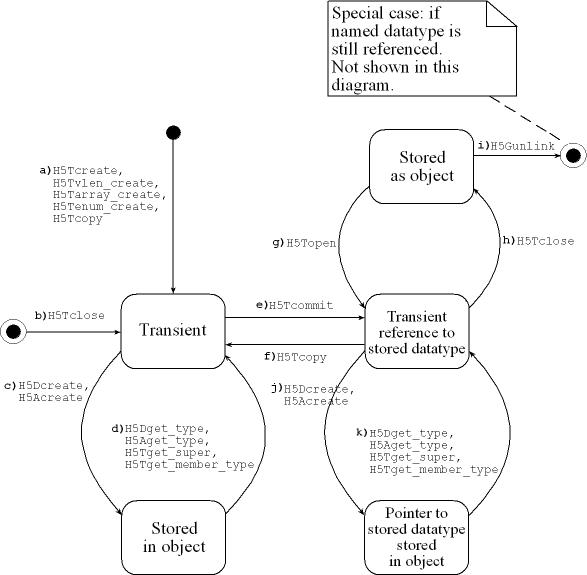
\includegraphics[scale=0.60]{images/datatype_life_cycle.png}
\caption{Datatype life cycle}
\label{fig:datatype-life-cycle}
\end{figure}

If a transient datatype is committed, the \texttt{vol\_obj} field of its shared information struct is populated with a copy of itself that is stored on disk, and the datatype's handle becomes a transient reference to the stored datatype. A transient reference to a stored datatype is also obtained when querying the datatype of an object with a committed datatype.

A committed datatype will be slated for removal from the file by \texttt{H5Ldelete} (or the deprecated \texttt{H5Gunlink}) if no other objects reference it. If it is unlinked and the objects that reference it are later deleted, the datatype's memory will be marked as free by the free space manager at that time. 

    \item Alignment

Different platforms may have different byte alignment restrictions when placing types within structures. The \texttt{HOFFSET} macro should be used when creating a compound type in order to align the inserted fields with any automatically added bytes of padding. 

Alignment of stored fields is not necessary when storing data structures on disk, and so the padding bytes can be removed to increase storage efficiency by `packing' the datatype. Compound types can be packed with \texttt{H5Tpack} to create storage-optimized unaligned versions. \texttt{H5Tpack} directly modifies the datatype it is given, so it should usually be preceded by \texttt{H5Tcopy}. Note that a packed datatype will usually be unable to describe in-memory data.

    \item Endianess
    
A platform that stores the most significant byte of a number at the smallest memory address is 'big-endian', and a platform that stores the least significant byte at the smallest memory address is 'little-endian.' The HDF5 library determines during its configuration which convention the current platform uses, and stores that as the 'native' convention, used by predefined types such as \texttt{H5T\_NATIVE\_INT}.
        
    \item Datatype hard and soft conversions

Each datatype conversion function has a 'hard' or 'soft' persistence. The persistence of a conversion function determines what source and destination datatypes it will be used for. A hard conversion function will only be used for the specific datatypes it is registered for, while a soft conversion function will be applied to any datatypes that match the classes of the source and destination types it is registered for.

A new hard conversion function will overwrite any previous conversion functions for the provided types, and a new soft conversion function will overwrite the conversion functions for any types to which it is applicable that do not already have a hard conversion function.
        
    \item Variable length datatypes

Because the total amount of storage space needed for objects with a variable length datatype cannot be known ahead of time and may change, data with a variable length type is stored in the file's global heap, rather than in the data object. The metadata describing the variable-length type itself is stored in a Datatype Message in an object's header, just as for non-variable-length datatypes. 

As a derived type, a variable-length datatype stores a pointer to its base datatype in the \texttt{parent} field of its shared type information structure. 

    \item Reference datatypes

Reference types are internally handled slightly differently than other 'complex' datatypes (e.g. compound, array, variable length types). Rather than having a unique structure which is a possible value of the union \texttt{u} in the shared type information structure, reference datatype objects are considered 'atomic', and are represented by a \texttt{H5T\_atomic\_t} instance. Reference-specific information is then stored under the \texttt{r} field of the atomic datatype structure's own union \texttt{u}.

    \item Datatype serialization

Datatype serialization to and from datatype messages is performed by the encode/decode callbacks on the datatype message class, \texttt{H5O\_\_dtype\_(encode/decode)}. It is also exposed as part of the API through \texttt{H5Tencode/H5Tdecode}. For atomic datatypes, encoding and decoding are accomplished non-recursively. For compound
types, a separate recursive call encodes each member field of the overall datatype. For arrays, variable-length types and enums a single recursive call is used to encode the base type.

    \item Addition of new native types
    
While the library allows applications to create their own custom datatypes, there are some reasons why a native datatype may be desired. For example, two applications may make different choices for how to implement complex numbers as a compound datatype, decreasing the portability of the data. For those interested in the process of introducing new native datatypes to the library, RFC THG 2015-04-29 ~\cite{rfc20150429}, specifically section 3.1, details which parts of the library and tools must be changed for compatibility with a new native datatype.

\end{itemize}

\subsection{Data Filters (\texttt{H5Z})}

%|  Name  | TODO | ONGOING | DONE |
%|--------|------|---------|------|
%| Dana   | x    |         |      |
%| Gerd   | x    |         |      |
%| Glenn  | x    |         |      |
%| Jordan | x    |         |      |
%| Luke   | x    |         |      |
%| Matt   |      |         |  x   |
%| Neil   | x    |         |      |
%| Scot   | x    |         |      |

\todo[inline]{Owner: Glenn -- Priority: Medium -- Effort: M -- Completion: 80\%}

\begin{itemize}
    \item Data filter pipeline

Data filters are used to manipulate data. The HDF5 library provides several built-in filters to allow for compression ({\footnotesize\texttt{H5Z\_FILTER\_DEFLATE}, \texttt{H5Z\_FILTER\_SZIP}, \texttt{H5Z\_FILTER\_NBIT}, \texttt{H5Z\_FILTER\_SCALEOFFSET}}), shuffling ({\footnotesize\texttt{H5Z\_FILTER\_SHUFFLE}}), and error checking ({\footnotesize\texttt{H5Z\_FILTER\_FLETCHER32}}). While filters can be used individually, they can also be stacked into a filter pipeline. Filters for contiguous datasets are not currently supported because implementing random access for partial I/O is difficult, and compact datasets are also not supported because the potential gains from filters are negligible on such small datasets. Theoretically, the maximum number of filter applications should be unlimited, but because each filter uses a bit in a 32-bit field, the actual maximum number of filter applications is 32. 

Users can also define their own filters to customize data processing further, which provides a high degree of flexibility for tailoring the pipeline to specific needs. As long as the filter is associated with a dataset upon the creation of that dataset, can be used with chunked data (\texttt{H5D\_CHUNKED}), and is applied to each individual chunk in a \texttt{H5D\_CHUNKED} dataset, then the custom filter may be registered and used. This is done through a two-step process. First, three callback functions must be written. The first is \texttt{H5Z\_can\_apply\_func\_t}, which checks against the dataset's dataset creation property list, datatype, and dataspace. The next is \texttt{H5Z\_set\_local\_func\_t}, which sets local flags and fields using the aforementioned three parameters. The last is \texttt{H5Z\_func\_t}, which takes in a bit vector of flags, the number of elements in the array of auxiliary data for the filter, the array of auxiliary data itself, the number of bytes in the filter buffer, the size of the filter buffer, and the filter buffer itself, and uses the fields set by the previous method to return the altered buffer back to the user along with its size. 

Once the above callbacks have been defined, the filter must be registered using \texttt{H5Zregister()}. \texttt{H5Zregister()} takes a pointer to a buffer for the class data structure and returns a \texttt{H5Z\_class\_t} (a two-byte identification number), which can be either \texttt{H5Z\_class1\_t} or \texttt{H5Z\_class2\_t}. 

\texttt{H5Z\_class\_t} is a macro that maps to either of the above two versions depending on the needs of the application. \texttt{H5Z\_class\_t}s start from 0-255, and these values are reserved for official HDF5 filters such as the ones listed above. 256-511 include the numbers that may be used for temporary testing. Lastly, 512-65535 is reserved for future assignments. If the filter is set as optional, then the library will skip the filter while proceeding through the filter pipeline.

At the center of the data filter pipeline is \texttt{H5Z\_pipeline()}, which is what carries out the pipeline. This method processes filters in definition order, or reverse order if the \texttt{H5Z\_FLAG\_REVERSE} flag is set. It takes in a \texttt{H5O\_pline\_t}, an unsigned int for flags, an array of unsigned ints for a filter mask, a \texttt{H5Z\_EDC\_t}, an \texttt{H5Z\_cb\_t} instance, a \texttt{size\_t} nbytes, which holds the number of bytes to filter, a \texttt{size\_t} buf\_size, which holds the total allocated size of the buffer, and buf, which is the buffer itself. This method will first check if the filter is registered, and if it is not already registered, it will try to load it dynamically and then register it. Once this is done, it will go through the list of filters in definition order and attempt to apply each filter to the data.

It is important to note that functions that allocate and free memory must be treated with care, since if there is a mismatch between the memory allocators used in the library and any memory that might be moved around by a filter, there may be problems. This issue can be resolved via the \texttt{H5allocate\_memory} and \texttt{H5free\_memory} functions, but if these methods are used, then the filter would have to be linked to a specific library version, which may be problematic. 

    \item Data transforms

Data transforms are also included in \texttt{H5Z}, and can be accessed via methods like \texttt{H5Z\_xform\_eval} on trivial transformations or \texttt{H5Z\_\_xform\_eval\_full} on complex transformations. This is done through the use of \texttt{H5Z\_node} to hold the parse tree and \texttt{H5Z\_token} to hold the original expression, current token values, and previous token values. Each \texttt{H5Z\_node} contains a left child, right child, \texttt{H5Z\_token\_type} to hold the type, and a \texttt{H5Z\_num\_val} to hold the value. Additionally, it includes macros for several different operations such as \texttt{H5Z\_XFORM\_DO\_OP1}, each of which is used in \texttt{H5Z\_\_xform\_reduce\_tree} to simplify parse trees, which is used when evaluating transformations.

\end{itemize}

\subsection{Dataspaces (\texttt{H5S})}

%|  Name  | TODO | ONGOING | DONE |
%|--------|------|---------|------|
%| Dana   | x    |         |      |
%| Gerd   | x    |         |      |
%| Glenn  | x    |         |      |
%| Jordan | x    |         |      |
%| Luke   | x    |         |      |
%| Matt   |      |         |  x   |
%| Neil   | x    |         |      |
%| Scot   | x    |         |      |

%\todo[inline]{Owner: Neil -- Priority: High -- Effort: L  -- Completion: 100\%}

A dataspace in HDF5 consists of two parts: an extent and a selection within that extent. They are mostly handled separately in the HDF5 library and only tied together at the top level of the structure. Extents are fairly trivial, consisting of a rank (number of dimensions) and size in each of these dimensions.

Selections are handled inside the \texttt{H5S} (dataspace) package with a flexible, class-like interface consisting of a \texttt{struct} of function pointers which must be implemented by each selection type. Currently, four selection types are implemented in HDF5: none, all, hyperslab, and point. `None' refers to a selection with no elements selected, while `all' refers to a selection of every element in the extent. Hyperslab selections are created using combinations of (\texttt{N}-dimensional) rectangular blocks, and a point selection is a list of individual elements. Point selection is the only selection type where the elements may be selected out of order, that is, the order of elements within the selection might not match the order of those elements within the serialized extent. Hyperslab blocks may be added in any order, but after combination, the order of the elements within the selection matches the order within the extent, as shown in Figure~\ref{fig:serial-offsets}. The order of elements within the extent is the same as the ordering of memory elements in a multi-dimensional array for the programming language used. Examples in this section use row-major ordering, as used by C.

\begin{figure}[h]
\centering
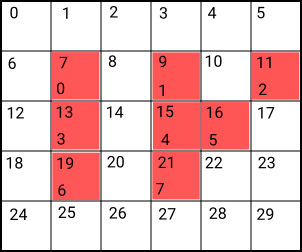
\includegraphics[scale=0.8]{images/Dataspace_serial_offsets.png}
\caption{A dataspace extent and selection (red) within the extent. The serialized offset within the extent is in the upper left of each element and the serialized offset within the selection is in the lower left.}
\label{fig:serial-offsets}
\end{figure}

\begin{itemize}
    \item Dataspace in-memory objects

The dataspace object in HDF5 is represented with the struct \texttt{H5S\_t} containing two fields, \texttt{extent} and \texttt{selection}, exactly mirroring the conceptual model above.

The extent field contains the dataspace extent (number of dimensions and number of elements in each dimension), as well as the type of extent, number of elements (for convenience), and information needed to encode the extent to an object header message.

The selection field contains the selection class (type) struct, which consists of a list of function pointers that the selection class uses to implement the necessary selection callbacks. The selection field also contains information on the selection offset, number of elements selected (again for convenience), and the information describing the actual shape of the selection, which depends on the selection class.

    \item Dataspace extents

Dataspace extents can be one of three types: scalar (\texttt{H5S\_SCALAR}), simple (\texttt{H5S\_SIMPLE}), and null (\texttt{H5S\_NULL}). A scalar dataspace extent represents a single element, a simple dataspace extent represents an N-dimensional array of elements, where N is between 1 and 32, and a null dataspace represents no elements. Simple dataspaces have an array size in each dimension, and also a maximum array size in each dimension (or \texttt{H5S\_UNLIMITED} to represent no maximum size). The size of each dimension can be changed with a call to \texttt{H5Sset\_extent()}, though each dimension size cannot be set to larger than the corresponding maximum dimension size. The maximum dimension sizes and the rank (number of dimensions) cannot be changed.

    \item Dataspace selections

Dataspace selections are used to select a subset of elements within the dataspace extent. They can be used to perform an operation on these elements, or simply to describe the subset (such as with a region reference). There are multiple types of selections, each of which must be defined by implementing the selection class, consisting of a series of callback functions that must be implemented. In addition, there are other functions that deal with individual selection types directly (such as \texttt{H5Sselect\_hyperslab()}) or that deal with multiple selection types (such as \texttt{H5Sselect\_project\_intersection()}).

    \item Hyperslab selections

Hyperslab selections represent an N-dimensional hyperrectangle of elements within the extent (where N is equal to the rank of the extent), a regular pattern of these hyperrectangles, or a combination of multiple hyperrectangles and/or patterns.

Hyperslabs are primarily constructed through the API using \texttt{H5Select\_hyperslab()}, which takes, as parameters, \texttt{start}, \texttt{stride}, \texttt{count}, and \texttt{block}, all of which are arrays of length matching the rank of the dataspace extent. \texttt{start} indicates the element at which the hyperslab begins (i.e. the element closest to position 0 in each dimension). \texttt{stride} indicates the spacing between the starting position of regularly spaced blocks in each dimension. \texttt{count} indicates the number of regularly spaced blocks in each dimension. \texttt{block} indicates the size of each regularly spaced block. In addition, hyperslabs can be combined in different ways using the \texttt{op} parameter, potentially yielding hyperslabs that cannot be represented using a single set of \texttt{start}, \texttt{stride}, \texttt{count}, and \texttt{block} arrays.

Internally, hyperslabs are represented in one of two ways. Hyperslabs that can be represented using a single set of \texttt{start}, \texttt{stride}, \texttt{count}, and \texttt{block} arrays are called \textit{regular} hyperslabs and are represented using these arrays. Other, irregular, hyperslabs are represented using a data structure called a \textit{span tree}.

A span tree is a multidimensional linked-list representing spans of selected elements. It is implemented using the \texttt{H5S\_hyper\_span\_info\_t} and \texttt{H5S\_hyper\_span\_t} structs. The entry point for a span tree is a \texttt{H5S\_hyper\_span\_info\_t} which is the head of the linked list of spans (each represented by a \texttt{H5S\_hyper\_span\_t}) in the slowest changing dimension of the dataspace. Each span contains a \texttt{down} pointer to a \texttt{H5S\_hyper\_span\_info\_t} in the next fastest changing dimension.

To more easily understand span trees, it is useful to start at the fastest changing dimension. In this dimension, there are no \texttt{down} pointers, and each span consists only of a low and high bound (coordinates in the fastest changing dimension of the dataspace), and a pointer to the next span. This forms a one-dimensional pattern of "dashes". In the next dimension up, this process is repeated, except instead of each span selecting a list of elements, it selects a list of these dashed patterns. An example of a span tree representation of a selection in a 2-D dataset can be found in Figure~\ref{fig:span-trees}.

\begin{figure}[h]
\centering
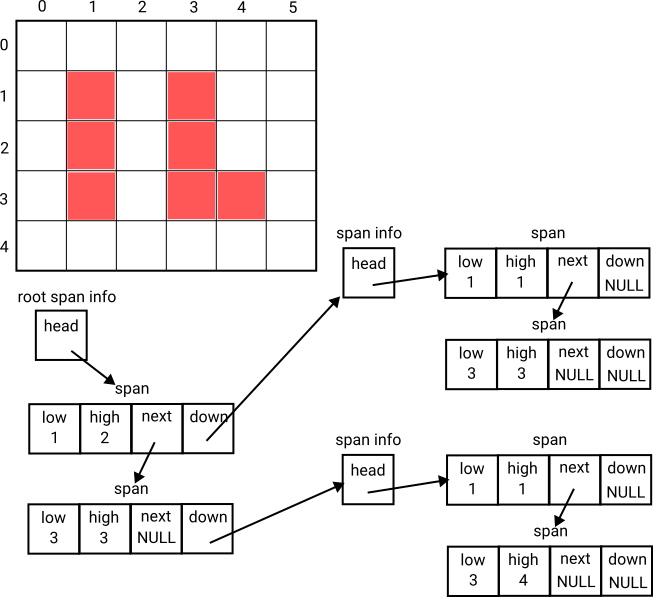
\includegraphics[scale=0.8]{images/Span_trees.png}
\caption{An illustration of span trees for a 2-D selection.}
\label{fig:span-trees}
\end{figure}

Hyperslabs can have either a regular description (start, stride, count, and block), a span tree description, or both.  Operations that are performed on hyperslabs need to be able to handle all of these cases. Some operations will construct a span tree for a regular on entry in order to simplify implementation (so it only needs to be implemented for span trees), though if an operation can be performed on a regular hyperslab directly that is generally more efficient. If a span tree is changed for a regular hyperslab it must be assumed it is no longer regular so the start, stride, block, and count are marked invalid. Also, after operations that can change a hyperslab, they will generally check if the hyperslab is regular and compute valid start, stride, block, and count values if so.

    \item Point selections

Point selections are a simple linear list of individual elements that are selected within the dataspace extent. They are implemented using a simple linked list of N-dimensional coordinates of each point. While conceptually simple, the fact that the points can be selected out of order with respect to the ordering of elements within the extent causes complications. The parallel code needs to take special care to reorder point selections as needed to obey MPI semantics, and virtual datasets do not support point selections at all. It is worth noting that it would not take much more work to implement point selection support for virtual datasets.

    \item Selection iterators and iteration operations

A selection iterator is a structure used to perform operations that iterate over a dataspace, such as generating offset/length pairs of selected elements (\texttt{H5S\_get\_seq\_list()}) or making a callback for each element selected (\texttt{H5S\_select\_iterate()}. The selection iterator includes another generic interface, \texttt{H5S\_sel\_iter\_class\_t}, that contains callback functions that must be implemented by each selection type. In addition, hyperslab and point selections store their own data in the selection iterator struct. These callbacks are used by the higher level code in \texttt{H5Sselect.c} to implement these operations. The iterator operations can also be called directly by external packages.

    \item Projections and the "shapesame" case

When performing I/O with selections, the library is given an extent and selection for the memory buffer, and a selection for the file (the extent for the file is implied by the dataset size). For contiguous datasets, the generic case here can be easily handled using selection iteration. The elements selected in the memory can be matched up 1-to-1 with elements selected in the file by the order within the selection, so the Nth element selected in memory is written to/read from the Nth element selected in the file. For chunked datasets, however, this becomes more complicated. The dataset in the file is broken up into chunks that may not be contiguous within the serialized (flattened) extent of the dataset, but the memory buffer is not broken up in the same way (indeed, the memory buffer need not have the same extent or even rank as the dataset). We therefore need to break the file selection up into a series of selections, one for each chunk. It is easy to do this using selection interfaces that compute the intersection of two selections. However, we also need to compute the selection in memory that corresponds to the selection within each chunk. Since the chunks may not be contiguous in the serialized extent, we can no longer rely on the 1-to-1 mapping used for contiguous datasets.

However, there is a shortcut we can take when a certain common condition is fulfilled. Often, the selections in the memory and file have the same shape, possibly with some offset between the two. If this is the case, we can simply, for each chunk, compute the intersection ("and") of that chunk with the file selection, then copy that intersection to the memory space, and apply any offset computed from comparing the overall file and memory selections. This copied intersection, called a projection, is now a selection containing the memory elements that match, in the correct order, the file elements selected that are in the current chunk. The dataset code then uses these file and memory chunk selection pairs to construct the I/O operation. The function used to check if two selections have the same shape is \texttt{H5S\_select\_shape\_same()} (wrapped by the macro \texttt{H5S\_SELECT\_SHAPE\_SAME()}), and the function used to construct the projected dataspace is \texttt{H5S\_select\_construct\_projection()}.

While the selections must have the same shape for this case to work, it is actually possible for the extents to be different ranks. If we have selections \(A\) and \(B\), with extents of rank \(M\) and \(N\), respectively, where \(M>N\), then \(A\) and \(B\) have the same rank if and only if selection \(A\) spans only a single element in the slowest changing \(M-N\) dimensions, and if \(A\) and \(B\) are identical in the fastest changing \(N\) dimensions, possibly with a constant offset. The library does not currently try to identify cases where the selections could be topologically identical by unrolling one or more dimensions, as this would require a different algorithm to construct the projection. They must actually be the same in the shared dimensions.

    \item The project intersection operation

The operation \texttt{H5Sselect\_project\_intersection()} and its corresponding private interface, \texttt{H5S\_select\_project\_intersection()}, is robust but can be confusing due to its complexity. This function takes three dataspaces, each with a selection, and outputs a fourth. Internally, this function is currently only used to implement virtual datasets, but it is also used by some VOL connectors to implement generic I/O with selections on chunked datasets. It may be beneficial in the future to implement chunked I/O using this operation when the shapesame case does not apply.

%\todo[inline]{GH: I think we should make a distinction between `chunks', which is a storage concept, and their counterparts in the dataspace context. How about we call them `tiles'? A tile is the logical place of a chunk in a dataspace. We definitely need a figure to show people an example of how the generic case falls apart.} 

In the general case for chunked dataset I/O we cannot simply copy the intersection from file to memory as in the shapesame case. The projected chunk selection in memory can be of a totally different shape from the chunk selection in the file. Instead, we can, for each chunk, calculate the offsets of the selected elements in that chunk within the serialized file selection, then select the elements in the memory space with the matching offsets within the serialized memory selection. This resulting memory chunk selection, which is a subset of the overall memory selection, contains the elements selected in the chunk being processed. An example showing this process for a single chunk of a two-dimensional dataset is shown in Figure~\ref{fig:project-intersection-chunk}. This process is repeated for every chunk that contains any selected elements. 

\begin{figure}[h]
\centering
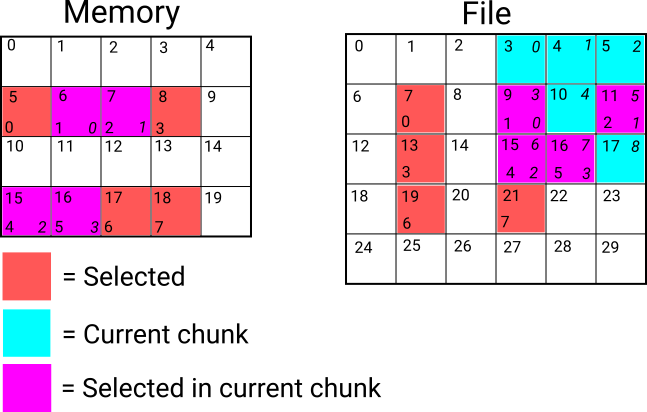
\includegraphics[scale=0.8]{images/Project_intersection_chunk.png}
\caption{A project intersection operation used for chunk I/O. The serialized offset within the extent is in the upper left of each element, the serialized offset within the selection is in the lower left, the serialized offset within the chunk is in the upper right, and the serialized offset within the intersected space is in the lower right. The result of the operation is the "selection in current chunk" (pink) in memory.}
\label{fig:project-intersection-chunk}
\end{figure}

The general chunked I/O case is supported by \texttt{H5S\_select\_project\_intersection()}, though that function also supports other use cases. \texttt{H5S\_select\_project\_intersection()} does not require that the selection representing the chunk in the above example be rectangular, it can be any selection that can be represented using the HDF5 API. In this function's terminology, the file selection (in the example) is referred to as the "source space", the memory selection is referred to as the "destination space", and the chunk selection is referred to as the "source intersect space". While the above description implies an element-by-element algorithm for calculating the source intersect space, in the case of hyperslabs (possibly combined with an all selection), the library uses span trees to be able to process the selection multiple elements at a time, which is generally much quicker. The project intersection operation can be thought of as projecting the intersection of the source space and the source intersect space onto the destination space, where there is a one-to-one mapping between the source space and the destination space (though they need not have the same shape).

This facility is not currently used by the native library to perform chunk I/O. If the shapesame case does not apply, the library iterates element by element over the selections in the dataset package. However, we would like to investigate using this function for the non-shapesame case in the native library, as we believe it may improve performance. The library currently uses this facility to implement virtual datasets, and some VOL connectors use it to implement chunked I/O. At some point in the future, we may wish to unify the shapesame projection and the project intersection operations.

    \item Parallel (MPI) operations

The dataspace code is also used to translate dataspace selections into MPI datatypes, which is central to the MPI I/O implementation. This functionality is present in \texttt{H5Smpio.c} and is called by functions in \texttt{H5Dmpio.c} as well as directly from the MPIO file driver in \texttt{H5FDmpio.c}. These functions are mostly straightforward, with different algorithms for point, regular hyperslab, and hyperslab span tree selections.

\end{itemize}

\subsubsection{Source files in the \texttt{H5S} package}

\begin{table}[!ht]
\begin{tabular}{||c|l||}
\hline
\textbf{Source File} & \textbf{Description} \\  [0.5ex] 
\hline\hline
\texttt{H5Spublic.h} & Public dataspace API \\
\texttt{H5Sprivate.h} & Private header (internal dataspace API) \\
\texttt{H5Spkg.h} & Package header (package private symbols) \\
\texttt{H5Smodule.h} & Package initialization boilerplate and User's Guide \\
\texttt{H5S.c} & Public API functions, package initialization, other core functions \\
\texttt{H5Sall.c} & `All' selection type \\
\texttt{H5Sdbg.c} & Debugging functions \\
\texttt{H5Sdeprec.c} & Deprecated functions \\
\texttt{H5Shyper.c} & `Hyperslab' selection type \\
\texttt{H5Smpio.c} & Parallel functionality for constructing MPI datatypes \\
\texttt{H5Sall.c} & `None' selection type \\
\texttt{H5Spoint.c} & `Point' selection type \\
\texttt{H5Sselect.c} & Operations on general hyperslab selections. Often just passes down to the specific selection type. \\  
\texttt{H5Stest.c} & Functions used only by the regression test suite \\
\hline
\end{tabular}
%\caption{}
\label{table:H5Scode}
\end{table}

%\subsubsection{Other source files referenced in this section}

%\begin{table}[h!]
%\begin{tabular}{||c|l||}
%\hline
%\textbf{Source File} & %\textbf{Description} \\  [0.5ex] 
%\hline\hline
%\texttt{H5Dmpio.c} & \ldots \\
%\texttt{H5FDmpio.c} & \ldots \\
%\hline
%\end{tabular}
%\caption{}
%\label{table:H5Smisc}
%\end{table}

% \subsection{References (\texttt{H5R})}
% \todo[inline]{Owner: ??? -- Priority: Low -- Effort: M}

\begin{comment}

\subsection{Property Lists (\texttt{H5P})}


%|  Name  | TODO | ONGOING | DONE |
%|--------|------|---------|------|
%| Dana   | x    |         |      |
%| Gerd   | x    |         |      |
%| Glenn  | x    |         |      |
%| Jordan | x    |         |      |
%| Luke   | x    |         |      |
%| Matt   | x    |         |      |
%| Neil   | x    |         |      |
%| Scot   | x    |         |      |

\todo[inline]{Owner: Dana -- Priority: Medium -- Effort: M -- Completion: 0\%}

\begin{itemize}
    \item Property list in-memory objects
    \item Property list classes and inheritance
    \item Property creation
    \item Setting and getting properties
    \item Property list serialization
\end{itemize}

% \subsection{Plugins (\texttt{H5PL})}
% \todo[inline]{Owner: Allen(?) -- Priority: Low -- Effort: S}

% There are three kinds of plugin in the library:

% \begin{itemize}
%     \item Filters
%     \item VOL connectors
%     \item VFD plugins
% \end{itemize}

% Each of these plugin categories is handled identically by the library, using a common plugin loading and caching harness.

% The plugin cache is so straightforward, it doesn't even warrant a drawing - it's just a simple collection of previously loaded plugin objects, each of which stores its category (e.g., filter), a unique key that can be used to identify the plugin (typically an integer ID, but might also be a name), and the plugin itself. When the library needs to search for a plugin, it simply checks the cache to see if the plugin has already been loaded, and, if not, tries to find and load the plugin via the plugin search path(s), storing it in the cache on success.

% The library also maintains a list of plugin paths. There is a platform-dependent default plugin path and API calls exist that allow users to manipulate the plugin path list. As with the plugin cache, the collection of plugin paths is common across all categories of plugins (though this may change in the future).

% Users can also set a plugin mask, which can be used to selectively disable plugin loads for each category of plugin. This mask is stored at the library level.

% The mechanism for creating an HDF5 library plugin is documented elsewhere. All plugins implement an interface (defined in H5PLextern.h) that allows the library to load and introspect plugins. Each category of plugins will additionally require the implementation of a number of callbacks.

% In the source code, plugins are handled via the H5PL package. Please see the package documentation in the repository for implementation details.
\end{comment}
\subsection{Virtual Object Layer (\texttt{H5VL})}\label{ref:vol}

%|  Name  | TODO | ONGOING | DONE |
%|--------|------|---------|------|
%| Dana   | x    |         |      |
%| Gerd   | x    |         |      |
%| Glenn  | x    |         |      |
%| Jordan | x    |         |      |
%| Luke   | x    |         |      |
%| Matt   | x    |         |      |
%| Neil   | x    |         |      |
%| Scot   | x    |         |      |

%\todo[inline]{Owner: Luke -- Priority: Medium -- Effort: L -- Completion: 100\%}

The virtual object layer (VOL) is an abstraction layer that intercepts all I/O-related calls in HDF5 and forwards them to custom callbacks. VOLs take as input high-level knowledge of the data format and data access characteristics, enabling the development of custom data operators, application-aware caching and logging, monitoring algorithms, specialized file formats, and integration with new storage technologies. Applications depending on HDF5 can leverage VOL plugins to meet their specific data requirements without code change through the use of environment variables and dynamic linking. This combination of extensibility and transparency positions HDF5 as an enduring data storage solution capable of adapting to a diversity of workloads and future innovations in storage technologies.

VOL connectors are highly flexible in the functionality they can encompass. Connectors can be applied in both serial and parallel HDF5, unlike VFDs. There are two general categories of VOL connector.
\begin{enumerate}
    \item \textbf{Pass-through VOL Connectors}: Forward data to a future VOL connector. An example is context-aware data caching which can intelligently place or prefetch data without change in the overall file format. Alternatively, an adaptive compression makes use of the data format to intelligently select a compression library. Note that HDF5 Filters have some similarities to pass-through connectors, but filters are limited to the native VOL. It is non-trivial to reuse filters in custom connectors. Other examples include the async and external VOLs in HDF5.
    \item \textbf{Terminal VOL Connectors}: The final VOL connector in a list of VOL connectors. Intended to be used for low-level data storage. An example is the HDF5 native VOL, which constructs the well-known HDF5 (*.hdf5) file format in storage. Other examples include the DAOS and S3 VOLs. Both DAOS and S3 are object stores, differing from traditional POSIX-compliant filesystems. HDF5 can now reliably store and retrieve data in these systems.
\end{enumerate}

VOL connector authors should be aware of the concurrency model of HDF5 when developing their VOLs:
\begin{enumerate}
    \item \textbf{Multi-Process Concurrency}: In parallel HDF5, Not all VOL functions are compatible with MPI\_Barrier. This is because not all I/O performed in HDF5 is collective. I/O is collective only when the application specifically passes H5FD\_MPIO\_COLLECTIVE flag or when the VOL function is related to internal HDF5 metadata updates.
    \item \textbf{Multi-Thread Concurrency}: VOL connectors will never be called from multiple threads at the same time in HDF5. This is because HDF5 uses a global lock when performing I/O. All VOLs in the list of VOLs will be executed in sequence before the lock is released. To improve concurrency, a VOL connector can leverage asynchronicity and internally spawn and manage its own worker threads for background tasks.
\end{enumerate}

\subsubsection{The VOL Class Structure}

VOL connectors are defined using the VOL class struct (\texttt{H5VL\_class\_t}), which contains function pointers to various HDF5 operation overrides and identifying information. VOLs are intended to follow the singleton design pattern. Typically the VOL class is declared as a static global variable in the VOL source file so that VOL functions can access the variable easily without explicitly passing it in. VOLs can choose to leave most functions unimplemented by setting them to NULL.

The VOL class has a few parameters regarding the identification and versioning of the VOL.
\begin{enumerate}
    \item \textbf{VOL connector ID}: A globally unique integer constant of type \texttt{H5VL\_class\_value\_t} that can be used to locate the VOL.
    \item \textbf{VOL name}: A globally unique semantic string that can be used to locate the VOL. While not technically erronous, spaces in the VOL name should be avoided since it increases the complexity of VOL initialization through environment variables.
    \item \textbf{VOL connector version}: An integer indicating the version of this VOL. This is mainly intended to help users ensure they are linking against the correct version of the VOL code.
    \item \textbf{VOL class struct version}: The version of the class struct being implemented. Different HDF5 versions have different class struct definitions. This allows HDF5 to determine whether the VOL was designed for the particular HDF5 version a user application is compiled against.
    \item \textbf{VOL capability flags}: Various flags indicating the supported functionality of the VOL. This can include information such as support for provenance, hard links and soft links, and attribute references.
\end{enumerate}

VOLs provide two functions for initializing and finalizing VOL classes.
\begin{enumerate}
    \item \textbf{initialize}: a method called to initialize the VOL connector
    \item \textbf{terminate}: a method called to free data allocated by VOL connector
\end{enumerate}

There are 9 general classes of functions that can be overridden for the HDF5 data model:
\begin{enumerate}
    \item \texttt{H5VL\_info\_class\_t}: Query the VOL connector's custom information. This can include methods for comparing two VOL connectors and allocating/freeing any custom state held by the VOL connector.
    \item \texttt{H5VL\_wrap\_class\_t}: Only for pass-through connectors. Used to manage the translation between the HDF5 library's internal representation of objects and the user's representation.
    \item \texttt{H5VL\_attr\_class\_t}: Override the HDF5 attribute APIs (H5A*), such as \texttt{H5Acreate}.
    \item \texttt{H5VL\_dataset\_class\_t}: Override the HDF5 dataset APIs (H5D*), such as \texttt{H5Dread}.
    \item \texttt{H5VL\_datatype\_class\_t}: Override the HDF5 datatype APIs (H5T*), such as \texttt{H5Tcreate}.
    \item \texttt{H5VL\_file\_class\_t}: Override the HDF5 file APIs (H5F*), such \texttt{H5Fcreate}.
    \item \texttt{H5VL\_group\_class\_t}: Override the HDF5 group APIs (H5G*), such as \texttt{H5Gcreate}.
    \item \texttt{H5VL\_link\_class\_t}: Override the HDF5 link APIs (H5L*), such as \texttt{H5Lexists}.
    \item \texttt{H5VL\_object\_class\_t}: Override the HDF5 object APIs (H5O*), such as \texttt{H5Ocopy}.
\end{enumerate}

There are 4 general classes of function that can be overridden relating to infrastructure/services:
\begin{enumerate}
    \item \texttt{H5VL\_introspect\_class\_t}: Container/connector introspection class callbacks.
    \item \texttt{H5VL\_request\_class\_t}: Asynchronous request class callbacks.
    \item \texttt{H5VL\_blob\_class\_t}: Blob class callbacks.
    \item \texttt{H5VL\_token\_class\_t}: VOL connector object token class callbacks.
\end{enumerate}

\subsubsection{VOL Registration}

It is mandatory for every VOL to implement and register the \texttt{H5VL\_class\_t} struct. This struct outlines the set of methods the VOL overrides. There are various ways to register the \texttt{H5VL\_class\_t} struct. In the library, there are three API routines for VOL registration:
\begin{enumerate}
    \item \texttt{H5VLregister\_connector}: takes as input the class struct pointer directly and registers it with HDF5
    \item \texttt{H5VLregister\_connector\_by\_name}: use the plugins interface (H5PL) to locate the VOL by the VOL name
    \item \texttt{H5VLregister\_connector\_by\_value}: use the plugins interface (H5PL) to locate the VOL by the connector ID
\end{enumerate}
During registration, the \texttt{initialize} function defined in the VOL class struct will be called if it is non-NULL. This function does not take any parameters -- except an empty property list. It is also only called once throughout the entire lifetime of the VOL and should be used to initialize any library or service required to be initialized exactly once. To pass variables to \texttt{initialize}, VOL authors should define custom environment variables and document them.

In addition, parameters can be passed to the VOL after registration using \texttt{H5VLconnector\_str\_to\_info}, which takes as input a string that is internally parsed by the VOL's custom \texttt{from\_str} function (defined in \texttt{H5VL\_info\_class\_t}). There is no required structure to this string, although it is best practice to avoid spaces and use `:'or `;' as separators for tokens. More complex parameters should be placed in custom environment variables instead. In \texttt{from\_str}, the parameter string will be parsed into a VOL-specific info struct, which can be accessed, copied, and queried using methods in \texttt{H5VL\_info\_class\_t}. An example of a parameter string to initialize a theoretical VOL named PFS that stores HDF5 data in a file on a PFS could be `username:/path/to/ssh/key:/path/to/file.txt'.

HDF5 can also transparently locate and register a VOL through the \texttt{HDF5\_PLUGIN\_PATH} and \\ \texttt{HDF5\_VOL\_CONNECTOR} environment variables. \texttt{HDF5\_PLUGIN\_PATH} tells HDF5 the directories to search for VOL libraries and \texttt{HDF5\_VOL\_CONNECTOR} holds a string containing the name and parameterization of a particular VOL to load. H5PL will split this string by spaces to determine the (VOL name, parameter) pair. Only a single VOL and its parameters can be specified using the environment variable. If the parameter string contains spaces, anything after the second space will be deleted. An example of \texttt{HDF5\_VOL\_CONNECTOR} for initializing the example PFS VOL could be `PFS username:/path/to/ssh/key:/path/to/file.txt', where PFS is the VOL name defined in the class struct. H5PL then automatically loads and registers the VOL, implicitly calling \texttt{H5VLregister\_connector\_by\_name} with the VOL name as input and \\ \texttt{H5VLconnector\_str\_to\_info} with the parameter string as input if it is not empty. \texttt{H5Pset\_vol} will then also be called to duplicate the info struct using the \texttt{copy} method defined in \texttt{H5VL\_info\_class\_t} and store in a property list tracked internally by HDF5. Generally, the info struct will be either passed directly to most VOL functions or queried from a property list.

To be compatible with H5PL, VOLs must implement the \texttt{H5PLget\_plugin\_type} and \\ \texttt{H5PLget\_plugin\_info} methods. HDF5 automatically searches for these methods and requires their signatures to be exactly correct. An example code is shown in Listing~\ref{lst:vol-init}.

\begin{listing}[!ht]
\centering
\caption{VOL plugin discovery code.}
\label{lst:vol-init}
\begin{minted}[linenos]{C}
static const H5VL_class_t H5VL_custom_vol_g = { /** method overrides */ }
H5PL_type_t H5PLget_plugin_type(void) {
  return H5PL_TYPE_VOL;
}
const void* H5PLget_plugin_info(void) {
  return &H5VL_custom_vol_g;
}
\end{minted}
\end{listing}

\subsubsection{VOL Organization}

\begin{figure}[!ht]
  \centering
  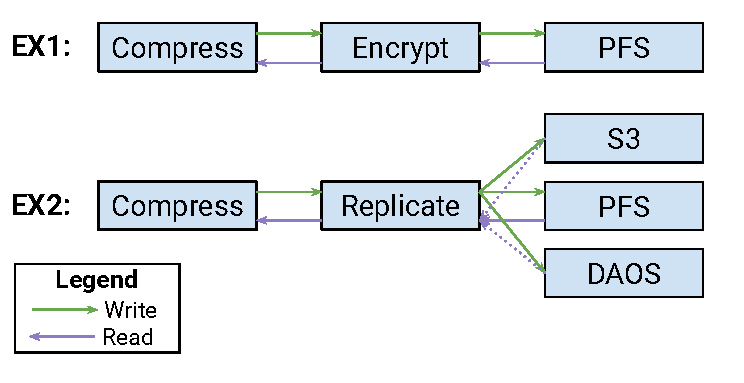
\includegraphics{images/tour_4_vol_dags.pdf}
  \caption{Depiction of data flow in VOL DAGs}
  \label{fig:vol-dag}
\end{figure}

VOLs can be conceptually organized as directed acyclic graphs (DAGs), although there is no specific DAG data structure in HDF5. Two examples of VOL DAGs and how data flows through them are shown in Figure~\ref{fig:vol-dag}. EX1 is a list of VOLs that compress, encrypt, and store the transformed data using a terminal PFS VOL. EX2 is a DAG of VOLs that compresses data and replicates the compressed data to numerous data repositories using terminal VOLs for S3, DAOS, and PFS. To create EX1, the parameter string would have to contain the information needed to register and initialize the compress, encrypt, and PFS VOLs. For example, \texttt{HDF5\_VOL\_CONNECTOR}=`compress zlib;encrypt:aes:/home/user/key.aes;PFS:/home/user/ex1.h5'. This string would be first passed to compress, where the relevant information needed to initialize the compress module will be parsed (zlib). Within the compress VOL, the name of the next VOL to create will be extracted (encrypt) and \texttt{H5VLregister\_connector\_by\_name} will be called using the remaining parameter string (aes:/home/user/key.aes;PFS:/home/user/ex1.h5). This will repeat recursively until each VOL is registered and defined. There is no specific functionality in HDF5 to initialize multiple VOLs at the same time -- it is the responsibility of a pass-through VOL developer to initialize any future VOLs it may depend on.

After initialization, I/O operations (e.g., dataset reads and writes) can be performed. Write operations are typically executed using preorder traversal (left-to-right for lists). For EX1, compression is first applied to the data, then encryption, and then persistent storage. EX2 is similar. Reads are typically executed using postorder traversal (right-to-left for lists). For EX1, data is first read from the PFS, decrypted, and then decompressed. In EX2, the replication VOL decides one of the three destinations (PFS, S3, or DAOS) to read data from, reads the data from that destination and then goes for decompression. In practice, these traversals are executed using recursion, where the first VOL registered is the root of the recursion. In EX1 and EX2, the root is the compress VOL. Pseudocode for the write and read operations for the compress VOL are depicted below in Listing~\ref{lst:compress-vol}. For writes, the input buffers stored in \texttt{buf} will be compressed into a new set of buffers \texttt{compressed}. The maximum size a compressed buffer can be is assumed to be the size of the original data, which is calculated using a custom \texttt{get\_data\_size} function. The compressed data is then forwarded to the next VOL using \texttt{H5VLdataset\_write}. Reads are similar, except the compressed data is first read using the next vol with \texttt{H5VLdataset\_read} and then decompressed into \texttt{buf}.

\begin{listing}[!ht]
\centering
\caption{Compression pass-through VOL code example.}
\label{lst:compress-vol}
\begin{minted}[linenos]{C}
typedef struct H5VL_compress_vol_info_t {
  int compress_method_;
  hid_t next_vol_id_;
  void *next_vol_info_;
} H5VL_compress_vol_info_t;
#define MAKE_TEMP_BUFFER \
  for (size_t i = 0; i < count; i++) { \
    next_objs[i] = objs[i]->next_vol_info_; \
    max_size[i] = get_data_size(mem_type_id[i], mem_space_id[i]); \
    compressed[i] = malloc(max_size[i]); \
  }
static herr_t H5VL_compress_vol_dataset_write(
    size_t count, void *dset[], hid_t mem_type_id[], hid_t mem_space_id[],
    hid_t file_space_id[], hid_t plist_id, const void *buf[], void **req) {
  H5VL_compress_vol_info_t **objs = (H5VL_compress_vol_info_t**)dset;
  void* next_objs[count]; void *compressed[count]; size_t max_size[count];
  MAKE_TEMP_BUFFER
  for (size_t i = 0; i < count; i++)
    compress(objs[i]->compress_method_, buf[i], max_size[i], compressed[i]);
  hid_t ret_value = H5VLdataset_write(
    count, (void**)next_objs, objs[0]->next_vol_id_, mem_type_id, 
    mem_space_id, file_space_id, plist_id, compressed, req);
  // Free compressed & return
}
static herr_t H5VL_compress_vol_dataset_read(/** Similar to write */) {
  H5VL_compress_vol_info_t **objs = (H5VL_compress_vol_info_t**)dset;
  void* next_objs[count]; void *compressed[count]; size_t max_size[count];
  MAKE_TEMP_BUFFER
  hid_t ret_value = H5VLdataset_read(/** Same as write */);
  for (size_t i = 0; i < count; ++i)
    decompress(objs[i]->compress_method_, compressed[i], max_size[i], buf[i]);
  // Free compressed & return
}
\end{minted}
\end{listing}


\subsubsection{Async VOLs}

VOLs can internally spawn thread pools to perform asynchronous operations and remove overhead such as locking and I/O stalls from the critical path. HDF5 does not provide a thread pool API and expects users will use an external threading library, such as pthreads or Argobots. Many VOL functions such as \texttt{H5VLdataset\_write} are either synchronous or asynchronous depending on if an HDF5 request struct is passed to it. \texttt{H5VL\_request\_class\_t} contains methods for waiting, canceling, completing, and freeing async requests. The VOL can define a custom request struct, taking as input the HDF request struct, and return it from VOL functions that behave asynchronously.

\subsubsection{Introspecting VOLs}

The introspection API provided by VOLs (\texttt{H5VL\_introspect\_class\_t}) provides several abilities to query properties of the VOL. \texttt{get\_conn\_cls} provides the ability to locate the class struct pointer for a VOL. The capability flags can be queried with \texttt{get\_cap\_flags}. Lastly, the \texttt{opt\_query} function allows for determining whether or not optional operations are supported by this VOL connector, such as a particular method in the \texttt{H5VL\_attr\_class\_t} struct. This is typically more fine-grained than the capability flag query. In addition, the \texttt{H5VL\_info\_class\_t} provides the ability to query the VOL's specific info struct, if the VOL defines one. The function \texttt{from\_str} allows the info struct to be converted into a human-readable string.

\subsubsection{Source files for \texttt{H5VL} developers}

\begin{table}[!ht]
\begin{tabular}{||c|l||}
\hline
\textbf{Source File} & \textbf{Description} \\  [0.5ex] 
\hline\hline
\texttt{H5VLpublic.h} & Public APIs for VOL registration and introspection \\
\texttt{H5VLconnector.h} & Public structs and APIs for VOL developers \\
\texttt{H5VLconnector\_passthru.h} & Public APIs for pass-through VOL developers \\
\texttt{H5VLpkg.h} & Internal APIs for VOL registration \\
\texttt{H5VLprivate.h} & Internal APIs for VOL calls \\
\texttt{H5VLmodule.h} & Internal macros for VOLs and documentation \\
\texttt{H5VL.c} & Implementation of H5VLpublic.h \\
\texttt{H5VLcallback.c} & Implementation of H5VLconnector.h and H5VLconnector\_passthru.h \\
\texttt{H5VLint.c} & Implementation of initialization functions in H5VLpkg.h \\
\texttt{H5VLdyn\_ops.c} & Implementation of optional functions in H5VLpkg.h \\
\texttt{H5VLtest.c} & Internal helpers for environment variable checks \\
\hline
\end{tabular}
%\caption{}
\label{table:VOL_src_files}
\end{table}

% \subsection{Event Sets and Asynchronous I/O (\texttt{H5ES})}
% \todo[inline]{Owner: ??? -- Priority: Medium -- Effort: S -- Completion: 0\%}

% \subsection{Minor/Convenience Interfaces (\texttt{H5[CS,RS,SL,UC,VM,WB]})}
% \todo[inline]{Owner: ??? -- Priority: Low -- Effort: M}

% \begin{itemize}
%     \item Skip lists (\texttt{H5SL})
%     \item Reference counted objects (\texttt{H5UC})
%     \item Reference counted strings (\texttt{H5RS})
%     \item Wrapped buffers (\texttt{H5WB})
%     \item Vector math (\texttt{H5VM})
%     \item Code stack (\texttt{H5CS})
% \end{itemize}
